% Biên dịch: pdflatex -shell-escape report.tex (minted cần -shell-escape), chạy 2 lần để có mục lục.
% Overleaf: Menu -> Compiler: pdfLaTeX (Overleaf tự bật shell-escape).
\documentclass[final]{hcmut-report}
\usepackage{codespace}

% Encodings
\usepackage{gensymb,textcomp}

% Better tables
\usepackage{array,longtable,multicol,multirow,siunitx,tabularx}

% Better enum
\usepackage{enumitem}
% Kiểu danh sách giống Khoi.zip: gạch ngang, dấu cộng, dấu sao; khoảng cách gọn
\setlist[itemize,1]{leftmargin=1.5em,itemsep=2pt,topsep=4pt,parsep=0pt,label={--}}
\setlist[itemize,2]{leftmargin=1.4em,itemsep=1pt,topsep=2pt,parsep=0pt,label={+}}
\setlist[itemize,3]{leftmargin=1.3em,itemsep=1pt,topsep=1pt,parsep=0pt,label={*}}

% Tiêu đề \paragraph dạng khối in đậm (như Khoi.zip)
\usepackage{titlesec}
\setcounter{secnumdepth}{3} % \paragraph không đánh số (tài liệu không dùng \subsubsection)
\titleformat{\paragraph}[block]{\normalfont\normalsize\bfseries}{\theparagraph}{1em}{}
\titlespacing*{\paragraph}{0pt}{1.5ex}{1ex}
\usepackage{needspace}

% Graphics
\usepackage{caption,float}
\usepackage[export]{adjustbox}

% Đồ thị cwnd vẽ trực tiếp từ dữ liệu đo (data/*.dat)
\usepackage{pgfplots}
\pgfplotsset{compat=1.17}
% Cache hình TikZ/pgfplots vào tikz-cache/ (cần -shell-escape); \cachedtikz{tên}{tikzpicture} đặt tên file cache
\usetikzlibrary{external}
\tikzexternalize[prefix=tikz-cache/]
\newcommand{\cachedtikz}[2]{\tikzsetnextfilename{#1}#2}
\usetikzlibrary{arrows.meta,positioning,shapes.multipart,fit,calc,decorations.pathreplacing}

% References
\usepackage[nameinlink]{cleveref}
\crefname{section}{mục}{mục}\Crefname{section}{Mục}{Mục}
\crefname{subsection}{mục}{mục}\Crefname{subsection}{Mục}{Mục}
\crefname{figure}{hình}{hình}\Crefname{figure}{Hình}{Hình}
\crefname{table}{bảng}{bảng}\Crefname{table}{Bảng}{Bảng}
\crefname{lstlisting}{đoạn mã}{đoạn mã}\Crefname{lstlisting}{Đoạn mã}{Đoạn mã}
\crefname{appendix}{phụ lục}{phụ lục}\Crefname{appendix}{Phụ lục}{Phụ lục}

% Configurations
\coursename{Mạng máy tính (CO3093)}
\reporttype{Báo cáo Bài tập lớn 1}
\title{Ứng dụng cộng tác client--server dựa trên streaming, chạy trên giao thức tin cậy tự thiết kế trên UDP}
\advisor{& ThS. Bùi Xuân Giang &}
\stuname{%
  & Phan Hải Phong &  \\
  & Trần Duy Phước Nghĩa &  \\
}
\reportplace{TP. Hồ Chí Minh}
\reporttime{Tháng 11/2026}

\AtBeginDocument{\counterwithin{lstlisting}{section}}
\AtBeginDocument{\renewcommand*{\lstlistlistingname}{Danh sách đoạn mã}}
\AtBeginDocument{\renewcommand*{\lstlistingname}{Đoạn mã}}

% Định nghĩa ngôn ngữ Go cho listings (listings không có sẵn Go)
\lstdefinelanguage{Go}{
  morekeywords={break,case,chan,const,continue,default,defer,else,fallthrough,for,func,go,goto,if,
    import,interface,map,package,range,return,select,struct,switch,type,var,nil,true,false},
  morekeywords=[2]{bool,byte,error,float64,int,int64,string,uint16,uint32,uint64,append,len,make,max,min,delete},
  sensitive=true,
  morecomment=[l]{//},
  morecomment=[s]{/*}{*/},
  morestring=[b]",
  morestring=[b]`,
}
\lstset{language=Go,basicstyle=\color{codebasic}\ttfamily\footnotesize}

% Hộp đánh dấu phần chưa viết của thành viên B (xóa khi đã điền nội dung)
\newcommand{\phanB}[1]{%
  \begin{center}
    \fcolorbox{red!70!black}{red!5}{\parbox{0.92\linewidth}{\textbf{[Phần của B]} #1}}
  \end{center}}

% Đường dẫn file / tên hàm trong code
\newcommand{\fname}[1]{\texttt{#1}}

% Cột bảng canh trái, tự xuống dòng (tránh khoảng trắng giãn ở cột hẹp)
\newcolumntype{L}[1]{>{\raggedright\arraybackslash}p{#1}}
\newcolumntype{Y}{>{\raggedright\arraybackslash}X}

% Cho phép giãn dòng thêm một chút để tên hàm dài (\texttt) không tràn lề
\setlength{\emergencystretch}{2em}
\AtBeginDocument{\renewcommand*{\refname}{Tài liệu tham khảo}}

\begin{document}
\coverpage%

\section*{Danh sách thành viên \& Phân công}
\begin{center}
  \begin{tabularx}{\linewidth}{clcY}
    \toprule
    \textbf{STT} & \textbf{Họ và tên} & \textbf{MSSV} & \textbf{Phụ trách} \\
    \midrule
    1 & Trần Duy Phước Nghĩa & 2412275 & \textbf{BTL 1} - \fname{internal/protocol} (gói, frame, tầng app), \fname{internal/transport} (truyền tin cậy, mã hóa, CUBIC, không HoL), tài liệu giao thức, test transport \\
    2 & Phan Hải Phong & 2412650 & \textbf{BTL 1} - \fname{internal/server} (handshake, đăng nhập, định tuyến, chuyển tiếp file),\fname{internal/client}, \fname{internal/webui}, test hệ thống \\
    3 & Bùi Trinh Nguyên Khải &   &   \\
    4 & Ngô Diệu Vy &   &   \\
    5 & Bùi Đăng Khoa &   &   \\
    \bottomrule
  \end{tabularx}
\end{center}
\clearpage

\tableofcontents
\listoffigures
\listoftables
\lstlistoflistings{}

\clearpage
\section{Tổng quan}
\label{sec:tong-quan}

\subsection{Bài toán}
Đề bài yêu cầu xây dựng một ứng dụng cộng tác theo mô hình client--server hoạt động trong mạng nội bộ (LAN).
Người dùng có thể đăng nhập, xem danh sách những người đang online, chat chung với cả phòng (broadcast), nhắn
tin riêng cho từng người (unicast) và gửi file cho nhau.

Yêu cầu trọng tâm và cũng là phần thử thách nhất của đề là toàn bộ dữ liệu phải truyền qua \textbf{một giao thức
tầng ứng dụng do nhóm tự thiết kế trên nền UDP}. Vì UDP vốn chỉ gửi từng gói tin (datagram) rời rạc, không đảm
bảo gói tới đích và cũng không giữ thứ tự, nhóm cần tự xây dựng thêm các cơ chế ở tầng trên để đáp ứng:
\begin{itemize}
  \item Truyền dữ liệu tin cậy và đúng thứ tự;
  \item Flow control -- tránh gửi nhanh hơn khả năng xử lý của bên nhận và Congestion control -- điều chỉnh tốc độ gửi theo tình trạng đường truyền, cài đặt thuật toán CUBIC \cite{rfc9438} hoặc BBR \cite{bbr};
  \item Mã hóa và xác thực dữ liệu trên đường truyền;
  \item Loại bỏ \emph{Head-of-Line blocking} (HoL), tức là khi đang truyền một file lớn thì các tin nhắn chat gửi xen kẽ không bị kẹt lại chờ file truyền xong.
\end{itemize}

\subsection{Lựa chọn công nghệ}
Nhóm hiện thực toàn bộ hệ thống bằng ngôn ngữ \textbf{Go} và \textbf{chỉ sử dụng thư viện chuẩn} (standard
library). Các package chính được dùng gồm:
\begin{itemize}
  \item \fname{net}: mở và đọc/ghi trực tiếp trên socket TCP, UDP thô (\fname{net.ListenUDP},
        \fname{WriteToUDP}, \fname{ReadFromUDP}).
  \item \fname{crypto/ecdh}, \fname{crypto/aes}, \fname{crypto/cipher}, \fname{crypto/sha256}: thực hiện trao đổi
        khóa X25519 \cite{rfc7748} và mã hóa đối xứng AES-256-GCM \cite{gcm}.
  \item \fname{encoding/binary}, \fname{encoding/json}: đóng gói header/frame nhị phân và serialize các bản tin
        tầng ứng dụng dưới dạng JSON.
\end{itemize}
Lý do chính nhóm chọn Go là vì cơ chế goroutine rất nhẹ (mỗi goroutine lúc khởi tạo chỉ tốn vài KB stack). Nhờ đó nhóm có thể tách riêng các luồng đọc, ghi và quản lý trạng thái cho từng kết nối; ngay cả khi server chạy đồng thời 20 client thì tổng số goroutine cũng chỉ khoảng vài chục. Ngoài ra, cấu trúc \fname{select} kết hợp với channel của Go rất hợp để viết event loop cho giao thức mạng mà hạn chế phải dùng quá nhiều khóa \texttt{Mutex}, giảm hẳn nguy cơ deadlock hay race condition.

\subsection{Phân tầng}
Để đáp ứng yêu cầu tách bạch giữa xử lý mạng, logic nghiệp vụ và giao diện, nhóm chia mã nguồn thành bốn tầng như ở \cref{tab:tang}.

\begin{table}[H]
  \centering
  \caption{Các tầng của hệ thống}
  \label{tab:tang}
  \begin{tabularx}{\linewidth}{lL{0.3\linewidth}Y}
    \toprule
    \textbf{Tầng} & \textbf{Package} & \textbf{Nhiệm vụ} \\
    \midrule
    Giao diện & \fname{internal/webui} & HTTP/1.1 cài đặt trên socket TCP, phục vụ trang HTML + JS thuần \\
    Ứng dụng & \fname{internal/server}, \fname{internal/client} & Xác thực đăng nhập, quản lý phiên online, định
    tuyến chat/DM, chuyển tiếp file \\
    Định dạng & \fname{internal/protocol} & Định nghĩa header gói, các loại frame, bản tin ứng dụng (\fname{AppMsg},
    \fname{FileMeta}) và bộ đệm sắp thứ tự \fname{SeqBuffer} \\
    Transport & \fname{internal/transport} & Truyền tin cậy trên UDP, mã hóa, ghép kênh nhiều stream độc lập,
    điều khiển luồng và tắc nghẽn \\
    \bottomrule
  \end{tabularx}
\end{table}

Giữa tầng ứng dụng và tầng transport, nhóm giao tiếp thông qua một interface chung là \fname{transport.Endpoint}
(\cref{sec:api}). Nhờ lớp trừu tượng này, phần code ở \fname{server} và \fname{client} chỉ cần gọi hàm gửi một
bản tin ngắn, mở một stream dài để truyền file, hoặc đọc các mảnh byte đã được sắp xếp đúng thứ tự từ channel
nhận về. Toàn bộ phần việc nặng ở dưới như chia nhỏ gói tin, đánh số thứ tự, gửi ACK, truyền lại gói mất hay mã
hóa đều được gói gọn bên trong \fname{internal/transport}.

\subsection{Đối chiếu với 10 bước của đề}
\label{subsec:rubric}

\begin{longtable}{c L{0.2\linewidth} L{0.42\linewidth} L{0.2\linewidth}}
  \caption{Đối chiếu 10 bước của đề với thiết kế}\label{tab:rubric} \\
  \toprule
  \textbf{Bước} & \textbf{Yêu cầu} & \textbf{Cách đáp ứng} & \textbf{Ở đâu} \\
  \midrule
  \endfirsthead
  \toprule
  \textbf{Bước} & \textbf{Yêu cầu} & \textbf{Cách đáp ứng} & \textbf{Ở đâu} \\
  \midrule
  \endhead
  1 & Thiết kế giao thức & Gói UDP $\le$ 1200 byte, 4 loại frame, ghép kênh nhiều stream trong một kết nối,
  phân loại stream MESSAGE và FILE & \cref{sec:giao-thuc} \\
  2 & Handshake TCP & Chuỗi bản tin \texttt{HELLO} $\to$ \texttt{KEYX} $\to$ \texttt{AUTH} $\to$
  \texttt{AUTH\_OK}/\texttt{AUTH\_FAIL} đóng khung \texttt{[len][JSON]}; mỗi phiên handshake chạy trên một
  goroutine riêng với deadline 10 s & \cref{subsec:handshake}, \cref{fig:seq-login} \\
  3 & Đăng nhập, quản lý trạng thái & File \texttt{users.json} chỉ lưu \texttt{sha256(salt $\|$ pass)};
  \fname{Registry} dùng \texttt{RWMutex} tra cứu session theo username và \texttt{conn\_id}, chặn đăng nhập
  trùng ngay trong lúc giữ khóa; server tự ghi đè trường \texttt{From} để chống giả mạo; tự động broadcast lại
  danh sách online khi có người vào/ra & \cref{sec:kien-truc}, \cref{sec:bao-mat} \\
  4 & Concurrency & Transport: mỗi kết nối có đúng 1 goroutine giữ state, giao tiếp qua channel. Server: mỗi
  session tách riêng goroutine đọc (\fname{serveSession}) và goroutine ghi (\fname{writeLoop}) kèm hàng đợi
  riêng, tránh việc một client đọc chậm làm nghẽn cả server; chạy ổn định với 20 client đồng thời
  (\cref{tab:he-thong}) & \cref{subsec:concurrency}, \cref{sec:kien-truc} \\
  5 & Streaming nhạy thời gian & Mỗi tin nhắn đi trên 1 stream ưu tiên cao riêng biệt; loại bỏ HoL ở cả chiều
  gửi lẫn chiều nhận & \cref{sec:hol} \\
  6 & Truyền file tin cậy qua UDP & Cơ chế SACK, phát hiện mất gói theo 3 điều kiện, chỉ truyền lại đúng frame bị
  mất, ghép dữ liệu theo offset, kiểm tra toàn vẹn bằng SHA-256 đầu cuối & \cref{sec:tin-cay} \\
  7 & Resilience & Keep-alive 2 s, idle timeout 10 s, frame \texttt{CLOSE}, bỏ qua gói lỗi/giả mạo,
  RTO exponential backoff. Server bọc \texttt{recover()} cho từng session và dọn dẹp session an toàn. Client hỗ
  trợ tự kết nối lại (backoff 1--30 s) và bắt tín hiệu Ctrl+C để gửi \texttt{CLOSE} trước khi thoát
  & \cref{subsec:song-chet}, \cref{subsec:state} \\
  8 & Bảo mật & Trao đổi khóa ECDH X25519 kết hợp AES-256-GCM, gắn header làm AAD, đảm bảo nonce không trùng lặp
  & \cref{sec:bao-mat} \\
  9 & Giao diện HTTP + JS thuần & Tự cài đặt parser HTTP/1.1 trực tiếp trên \fname{net.Listen} (xử lý request
  line, header, \texttt{Content-Length}); giao diện HTML + JS thuần dùng cơ chế polling
  \texttt{/api/events?since=N}; upload file qua \texttt{POST} raw body; nhúng file tĩnh vào binary bằng
  \texttt{embed} & \cref{sec:kien-truc} \\
  10 & Test, chất lượng code & Kiểm tra \fname{go vet} và \fname{go test -race}; viết unit test cho
  protocol/transport, integration test cho server (\fname{FakePair}) và end-to-end test qua UDP thật với loss
  10\%; đo đạc hiệu năng trên bộ giả lập mạng & \cref{sec:kiem-thu} \\
  \bottomrule
\end{longtable}


\section{Kiến trúc hệ thống}
\label{sec:kien-truc}

Hệ thống gồm một server trung tâm và nhiều client. Vì trình duyệt web không mở được socket UDP thô, mỗi client chạy như một process cục bộ trên máy người dùng: trình duyệt giao tiếp với process client qua HTTP trên \texttt{127.0.0.1}, còn dữ liệu đi ra mạng LAN giữa client và server đi qua kênh UDP đã mã hóa (trừ bước handshake ban đầu dùng TCP để trao đổi khóa và đăng nhập). \Cref{fig:tong-quan} minh họa ba kênh mạng giữa các client và server; \cref{fig:kien-truc} trình bày các thành phần và luồng dữ liệu bên trong mỗi process.

\begin{figure}[tbp]
  \centering
  \begin{tikzpicture}[font=\small,
      br/.style={draw, rounded corners, fill=gray!8, align=center, minimum width=2.2cm, minimum height=0.9cm},
      cl/.style={draw, rounded corners, fill=blue!8, align=center, minimum width=2.6cm, minimum height=0.9cm},
      port/.style={draw, rounded corners, fill=orange!12, align=center, minimum width=2.9cm, minimum height=0.8cm},
      http/.style={<->, >={Stealth}, thick, gray!70!black},
      tcp/.style={->, >={Stealth}, thick, dashed, blue!60!black},
      udp/.style={<->, >={Stealth}, very thick, orange!80!black},
      disc/.style={->, >={Stealth}, thick, dotted, green!45!black},
      lab/.style={font=\scriptsize, fill=white, inner sep=1pt}]
    % clients
    \foreach \y/\n/\w in {2.2/alice/8081, 0/bob/8082, -2.2/carol/8083} {
      \node[br] (b\n) at (0,\y) {Trình duyệt\\\scriptsize HTML + JS};
      \node[cl] (c\n) at (4.6,\y) {Client \n\\\scriptsize process trên máy \n};
      \draw[http] (b\n) -- node[lab, above=2pt] {HTTP :\w} (c\n);
    }
    % server: draw the frame first so the port boxes sit on top of it
    \node[draw, thick, rounded corners, fill=green!5, minimum width=3.8cm, minimum height=4.4cm,
      label={[font=\small\bfseries]above:Server}] (srv) at (12,0) {};
    \node[port] (p9000) at (12, 1.4) {TCP :9000\\\scriptsize handshake, đăng nhập};
    \node[port] (p9001) at (12, 0)   {UDP :9001\\\scriptsize dữ liệu đã mã hóa};
    \node[port] (p9002) at (12,-1.4) {UDP :9002\\\scriptsize broadcast tìm server};
    \foreach \n in {alice, bob, carol} {
      \draw[tcp]  ([yshift=0.25cm]c\n.east) to[out=0, in=180] (p9000.west);
      \draw[udp]  (c\n.east) to[out=0, in=180] (p9001.west);
      \draw[disc] (p9002.west) to[out=180, in=0] ([yshift=-0.25cm]c\n.east);
    }
    % legend
    \begin{scope}[shift={(2.2,-3.5)}, font=\scriptsize]
      \draw[http] (0,0)    -- (0.8,0)    node[right, black] {HTTP cục bộ, chỉ trong máy người dùng};
      \draw[tcp]  (0,-0.4) -- (0.8,-0.4) node[right, black] {TCP: trao khóa X25519 và đăng nhập, đóng ngay sau đó};
      \draw[udp]  (0,-0.8) -- (0.8,-0.8) node[right, black] {UDP tin cậy tự viết: chat, DM, file, ACK, mã hóa AES-256-GCM};
      \draw[disc] (0.8,-1.2) -- (0,-1.2); \node[right] at (0.8,-1.2) {UDP broadcast mỗi 2 s, client dùng khi chạy \texttt{-server auto}};
    \end{scope}
  \end{tikzpicture}
  \caption{Tổng quan: nhiều client nối tới một server qua ba kênh mạng}
  \label{fig:tong-quan}
\end{figure}

\begin{figure}[tbp]
  \centering
  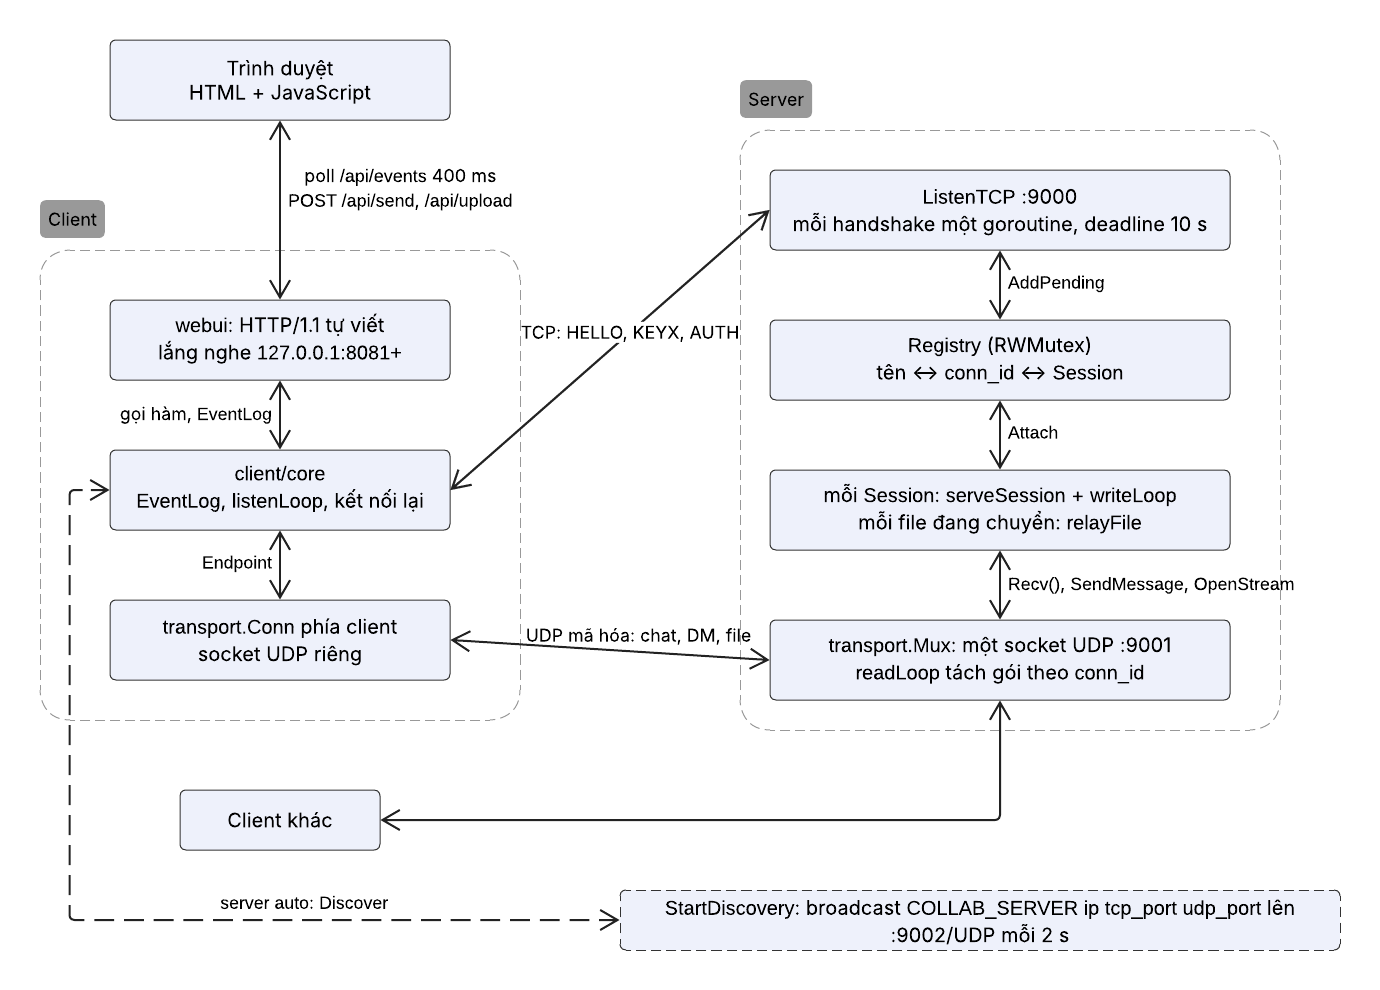
\includegraphics[width=\linewidth]{img/kien-truc.png}
  \caption{Kiến trúc chi tiết: các thành phần, goroutine chính và luồng dữ liệu}
  \label{fig:kien-truc}
\end{figure}

\paragraph{Phía Server.} Server chia thành ba nhóm goroutine chính:
\begin{enumerate}[label=(\arabic*), leftmargin=*, itemsep=2pt]
  \item \fname{ListenTCP} lắng nghe trên cổng 9000; mỗi lượt handshake chạy trong một goroutine riêng với deadline
        10 giây. Ngay sau khi xác thực thành công, server gọi \fname{Mux.Accept(conn\_id, $k_\text{udp}$)} để tạo
        đối tượng \fname{transport.Conn} cho kết nối UDP và gắn vào \fname{Session}.
  \item Mỗi session đang hoạt động có hai goroutine dài hạn: \fname{serveSession} đọc từ \texttt{Recv()} và phân
        loại stream theo byte đầu tiên (cắt tới cờ FIN rồi đưa đi định tuyến; luồng file được
        tách phần metadata ở đầu rồi chuyển tiếp từng mảnh sang goroutine \fname{relayFile} của file đó). Ở chiều
        ngược lại, \fname{writeLoop} là goroutine \emph{duy nhất} gọi \texttt{SendMessage} cho session này, lấy tin
        tuần tự từ hàng đợi \texttt{sendCh} (4096 phần tử) để giữ thứ tự gửi và cô lập các client nhận chậm
        (\cref{subsec:app}). Khi mới tạo phiên, một goroutine ngắn hạn \fname{watchPeer} chờ gói UDP đầu tiên của
        client để ghi nhận địa chỉ IP:port thực tế và phát lại danh sách user kèm địa chỉ mới cho cả phòng.
  \item \fname{Mux.readLoop} đọc gói từ socket UDP chung trên cổng 9001, tra trường \texttt{conn\_id} trong header
        để chuyển gói tới đúng đối tượng \fname{Conn}; mỗi \fname{Conn} có một goroutine \fname{run} riêng ở tầng
        transport.
\end{enumerate}
Danh sách người dùng online được lưu tại \fname{Registry} dưới khóa \texttt{RWMutex}. Các phương thức của
\fname{Registry} chỉ cập nhật hoặc chép nhanh danh sách (\fname{Snapshot}) rồi nhả khóa ngay trước khi gửi mạng,
tránh giữ khóa trong lúc I/O.

\paragraph{Phía Client.} Khi chạy với cờ \texttt{-server auto}, client lắng nghe gói UDP broadcast trên cổng 9002
(tối đa 5 giây) và lấy IP server từ địa chỉ nguồn của gói tin; socket bật \texttt{SO\_REUSEADDR}/\texttt{SO\_REUSEPORT}
để nhiều tiến trình client trên cùng máy có thể lắng nghe đồng thời. Khối \fname{client/core} giữ \fname{Endpoint}
hiện tại cùng goroutine \fname{listenLoop} ghép các stream nhận về, sắp lại thứ tự tin nhắn theo \texttt{Seq} và
ghi các sự kiện (chat, DM, danh sách user, tiến độ truyền file, trạng thái kết nối) vào \fname{EventLog} theo chỉ
số tăng dần. Nếu channel \texttt{Done()} đóng mà không do người dùng thoát, client chuyển sang trạng thái
\textsc{Reconnecting} và thực hiện handshake lại (\cref{subsec:state}).

\paragraph{Giao diện.} \fname{webui} là một HTTP/1.1 server nhóm tự viết trên \fname{net.Listen} (đọc request
line, header và body theo \texttt{Content-Length}), phục vụ trang HTML + JavaScript thuần nhúng sẵn vào file thực
thi. Trình duyệt poll \texttt{/api/events?since=N} để lấy sự kiện mới từ \fname{EventLog} (mỗi sự kiện có số thứ tự
tăng dần nên F5 hay mở nhiều tab không mất hoặc lặp tin) và \texttt{/api/status} để hiện RTT, cwnd, tỉ lệ mất gói.
File gửi đi được đẩy thẳng vào body của \texttt{POST /api/upload}. Luồng đi của một DM và một file qua các khối trên
được vẽ ở \cref{fig:seq-dm,fig:seq-file}; chi tiết cài đặt có trong \fname{docs/code-walkthrough.md}.
\IfFileExists{img/webui.png}{\Cref{fig:webui} là giao diện khi đang gửi file: cột trái là danh sách user
online kèm IP:port, giữa là tin nhắn theo tab (chat chung và từng DM) cùng thanh tiến trình file, thanh trên cùng
là trạng thái mạng (connected/reconnecting, RTT, cwnd, tỉ lệ mất gói).}{}

\IfFileExists{img/webui.png}{%
\begin{figure}[H]
  \centering
  \includegraphics[width=\linewidth]{img/webui.png}
  \caption{Giao diện web của client khi đang gửi file}
  \label{fig:webui}
\end{figure}}{}

\section{Đặc tả giao thức}
\label{sec:giao-thuc}

Giao thức gồm hai giai đoạn: \textbf{handshake trên TCP} (trao đổi khóa và đăng nhập, xong thì đóng) và
\textbf{truyền dữ liệu trên UDP} (chat, DM, file, ACK, keep-alive). Mọi số nguyên trên dây đều là
\emph{big-endian}. Định nghĩa đầy đủ nằm trong \fname{internal/protocol} và \fname{docs/protocol.md}.

\subsection{Cổng}
\begin{table}[H]
  \centering
  \caption{Các cổng sử dụng}
  \label{tab:cong}
  \begin{tabularx}{\linewidth}{llY}
    \toprule
    \textbf{Cổng} & \textbf{Giao thức} & \textbf{Dùng cho} \\
    \midrule
    9000 & TCP & Handshake: trao đổi khóa, đăng nhập (đóng sau khi xong) \\
    9001 & UDP & Toàn bộ dữ liệu: message, file, ACK, PING, CLOSE \\
    9002 & UDP broadcast & Server quảng bá địa chỉ trong LAN để client tự tìm \\
    8080+ & TCP (HTTP tự viết) & Web UI của từng client, chỉ lắng nghe trên \texttt{127.0.0.1} \\
    \bottomrule
  \end{tabularx}
\end{table}

\subsection{Handshake TCP}
\label{subsec:handshake}
Mỗi message handshake có dạng \texttt{[4 byte độ dài][JSON]}. Độ dài bị giới hạn 1 MB: độ dài do bên kia tự
khai, nếu không giới hạn thì kẻ xấu chỉ cần gửi độ dài 4 GB là làm server cấp phát hết bộ nhớ.

\begin{table}[H]
  \centering
  \caption{Các message handshake}
  \label{tab:handshake}
  \begin{tabularx}{\linewidth}{clL{0.2\linewidth}Y}
    \toprule
    \textbf{\#} & \textbf{Hướng} & \textbf{Message} & \textbf{Nội dung} \\
    \midrule
    1 & C $\to$ S & \texttt{HELLO} & \texttt{client\_pub}: khóa công khai X25519 (tạm, mỗi phiên một khóa) \\
    2 & S $\to$ C & \texttt{KEYX} & \texttt{server\_pub}, \texttt{conn\_id} (định danh kết nối UDP),
    \texttt{udp\_port} \\
    3 & C $\to$ S & \texttt{AUTH} & \texttt{nonce} 12 byte ngẫu nhiên, \texttt{sealed} =
    AES-GCM$_{k_\text{tcp}}$(\{user, pass\}) \\
    4 & S $\to$ C & \texttt{AUTH\_OK} / \texttt{AUTH\_FAIL} & danh sách user online / lý do từ chối \\
    \bottomrule
  \end{tabularx}
\end{table}

Sau bước 2, hai bên tự tính cùng một bí mật chung mà không ai gửi nó qua mạng, rồi tách ra hai khóa:
\begin{align}
  \mathit{shared} &= \mathrm{X25519}(\mathit{priv}, \mathit{peerPub}) \\
  k_\text{tcp} &= \mathrm{SHA256}(\mathit{shared} \,\|\, \texttt{tcp}) \quad
    \text{mã hóa user/password trong \texttt{AUTH}} \\
  k_\text{udp} &= \mathrm{SHA256}(\mathit{shared} \,\|\, \texttt{udp}) \quad
    \text{mã hóa mọi gói UDP}
\end{align}
Dùng hai khóa riêng để hai kênh có cách sinh nonce khác nhau (TCP: nonce ngẫu nhiên; UDP: nonce từ header) không
bao giờ dùng chung một khóa. Sau \texttt{AUTH\_OK}, kết nối TCP đóng; client gửi gói UDP đầu tiên (PING) mang
\texttt{conn\_id} để server biết địa chỉ UDP của mình.

\subsection{Gói UDP}
\label{subsec:goi}

\begin{figure}[H]
  \centering
  \begin{tikzpicture}[x=0.82cm,y=1cm,font=\small]
    \foreach \xa/\xb/\fld/\sub in {0/2/{magic}/{0xC0DE},2/3/{ver}/{1},3/4/{flg}/{},4/6.5/{conn\_id}/{uint32},
      6.5/9/{packet\_num}/{uint32}} {
      \draw[fill=blue!8] (\xa,0) rectangle (\xb,1);
      \node[font=\footnotesize] at ({(\xa+\xb)/2},0.65) {\texttt{\fld}};
      \node[font=\scriptsize] at ({(\xa+\xb)/2},0.25) {\sub};
    }
    \draw[fill=orange!10] (9,0) rectangle (14.5,1);
    \node at (11.75,0.65) {frame (đã mã hóa)};
    \node[font=\scriptsize] at (11.75,0.25) {$\le$ 1172 byte};
    \draw[fill=gray!15] (14.5,0) rectangle (16,1);
    \node at (15.25,0.5) {tag};
    \foreach \x/\l in {0/0,2/2,3/3,4/4,6.5/8,9/12} \node[font=\scriptsize,above] at (\x,1) {\l};
    \draw[decorate,decoration={brace,amplitude=5pt,mirror}] (0,-0.1) -- (9,-0.1)
      node[midway,below=6pt,font=\scriptsize] {header 12 byte: gửi rõ, là AAD của AES-GCM};
    \draw[decorate,decoration={brace,amplitude=5pt,mirror}] (14.5,-0.1) -- (16,-0.1)
      node[midway,below=6pt,font=\scriptsize] {16 byte};
  \end{tikzpicture}
  \caption{Cấu trúc một gói UDP (tổng $\le$ 1200 byte)}
  \label{fig:goi}
\end{figure}

\begin{itemize}
  \item \textbf{Kích thước $\le$ 1200 byte} để không bị phân mảnh IP trên mọi đường truyền (MTU tối thiểu của
        IPv6 là 1280 byte, trừ header IP/UDP), giống QUIC \cite{rfc9000}. Phần frame còn lại
        $1200 - 12 - 16 = 1172$ byte.
  \item \texttt{magic} và \texttt{ver} giúp loại nhanh gói không thuộc giao thức trước khi tốn công giải mã.
  \item \texttt{conn\_id} cho biết gói thuộc kết nối nào: server dùng chung một socket UDP cho mọi client và
        tra \texttt{conn\_id} để chuyển gói tới đúng kết nối, nên client đổi địa chỉ (NAT) vẫn nhận ra.
  \item \texttt{packet\_num} \textbf{tăng mãi, không bao giờ dùng lại}, kể cả khi gửi lại: dữ liệu của gói bị mất
        được đóng vào gói mới với số mới. Nhờ vậy mỗi ACK chỉ khớp đúng một lần gửi, đo RTT không bao giờ mập mờ
        (không cần thuật toán Karn như TCP), và nonce mã hóa không bao giờ lặp (\cref{sec:bao-mat}).
\end{itemize}

\subsection{Frame}
\label{subsec:frame}
Phần đã mã hóa của gói chứa một hoặc nhiều frame xếp liền nhau. Bên nhận đọc byte \texttt{type} để biết độ dài
frame, cắt ra, rồi đọc tiếp tới hết. Nhờ vậy một gói có thể vừa mang dữ liệu vừa mang ACK (\emph{piggyback}).

\begin{table}[H]
  \centering
  \caption{Bốn loại frame}
  \label{tab:frame}
  \begin{tabularx}{\linewidth}{clL{0.3\linewidth}cY}
    \toprule
    \textbf{Type} & \textbf{Tên} & \textbf{Cấu trúc (byte)} & \textbf{ACK?} & \textbf{Ý nghĩa} \\
    \midrule
    0x01 & STREAM & \texttt{type(1) flags(1) stream\_id(4) offset(4) len(2) data} & Có &
    1 đoạn dữ liệu ($\le$ 1000 byte) của 1 stream; bit 0 của \texttt{flags} = FIN \\
    0x02 & ACK & \texttt{type(1) window(4) n(1)} $n \times$ \texttt{[start(4) end(4)]} & Không &
    SACK theo \texttt{packet\_num} ($n \le 8$) + cửa sổ nhận \\
    0x03 & PING & \texttt{type(1)} & Có & Giữ kết nối, báo địa chỉ client cho server \\
    0x04 & CLOSE & \texttt{type(1) reason\_len(1) reason} & Không & Đóng ngay, không chờ timeout \\
    \bottomrule
  \end{tabularx}
\end{table}

\paragraph{STREAM.} Một \emph{stream} là một dãy byte có thứ tự (một tin nhắn, hoặc một file). Nhiều stream
chạy song song trong cùng một kết nối. \texttt{offset} là vị trí byte đầu tiên của \texttt{data} trong stream,
bên nhận ghép lại theo offset. Client đánh \texttt{stream\_id} lẻ (1, 3, 5\dots), server đánh số chẵn, nên hai
bên mở stream đồng thời cũng không bao giờ trùng số. Mỗi frame mang tối đa 1000 byte dữ liệu để gói còn chỗ ghép
thêm một ACK (tối đa 70 byte).

\paragraph{ACK.} Liệt kê các khoảng \texttt{packet\_num} đã nhận, sắp giảm dần, khoảng đầu tiên kết thúc ở gói
lớn nhất. Ví dụ đã nhận gói 1--5, 7--9 và 12:
\begin{center}
  \texttt{[0x02][window=48000][n=3][12,12][7,9][1,5]} \quad (30 byte; thiếu 6, 10, 11)
\end{center}
Đây là \emph{selective ACK}: bên gửi biết chính xác gói nào thiếu và chỉ gửi lại dữ liệu của gói đó.
\texttt{window} là số byte bên nhận còn trống, dùng cho điều khiển luồng (\cref{subsec:dieu-toc}).
Gói chỉ chứa ACK thì không được ACK lại, nếu không hai bên sẽ ACK qua lại vô hạn.

\paragraph{CLOSE.} \texttt{reason} là chuỗi UTF-8 tối đa 255 byte; bên gửi tự cắt nếu dài hơn, và cắt đúng
ranh giới ký tự để không làm hỏng ký tự nhiều byte.

\subsection{Nội dung stream (tầng ứng dụng)}
\label{subsec:app}
Byte đầu tiên của mỗi stream cho biết loại:
\begin{center}
  \small
  \begin{tabular}{ll}
    MESSAGE: & \texttt{[0x01][JSON AppMsg \dots{} tới hết stream]} \\
    FILE: & \texttt{[0x02][meta\_len u32][JSON FileMeta][dữ liệu file \dots]}
  \end{tabular}
\end{center}

\begin{lstlisting}[caption={Cấu trúc nội dung tầng ứng dụng (\fname{appmsg.go}, rút gọn)},
  label=lst:appmsg]
type AppMsg struct {
	Type  string   `json:"type"` // chat | dm | users | join | leave | error
	From  string   `json:"from,omitempty"`
	To    string   `json:"to,omitempty"`
	Text  string   `json:"text,omitempty"`
	Users []string `json:"users,omitempty"`
	TS    int64    `json:"ts"`            // UnixMilli
	Seq   uint64   `json:"seq,omitempty"` // per-connection message number
}

type FileMeta struct {
	ID, From, To, Name string
	Size   int64
	SHA256 string // hex; receiver re-hashes the file to verify it
}
\end{lstlisting}

Meta của file đi \textbf{chung stream} với dữ liệu file thay vì gửi bằng một message riêng, vì giữa các stream
không có thứ tự: nếu tách ra thì dữ liệu file có thể tới trước meta. Bên nhận đọc meta theo từng byte tới
(\fname{FileHeaderParser}), không cần chờ cả file. SHA-256 của toàn bộ file đi trong meta để bên nhận kiểm tra file
nguyên vẹn đầu cuối, độc lập với tầng transport.

\paragraph{Thứ tự tin nhắn (\texttt{Seq}).} Mỗi tin là một stream riêng để tin này không phải chờ tin kia
(\cref{sec:hol}); hệ quả là khi mất gói, tin \#2 có thể giao trước tin \#1. Để vẫn giao đúng thứ tự gửi, mỗi bên
gửi đánh \texttt{Seq} = 1, 2, 3\dots{} theo từng kết nối, và bên nhận dùng \fname{protocol.SeqBuffer}: tin tới
sớm được giữ lại tới khi các tin trước đủ, tin trùng bị bỏ, \texttt{Seq} = 0 được giao ngay. Nếu giữ quá 4096 tin
(chỉ xảy ra khi có lỗi) thì bỏ qua chỗ trống để không treo vĩnh viễn. File không cần cơ chế này vì mỗi file là
một stream, tầng transport đã giao đúng thứ tự theo offset.

\phanB{Mô tả cách client và server dùng \texttt{Seq}/\texttt{SeqBuffer} (đánh số ở đâu, hàng đợi gửi của server
xử lý thế nào khi đầy) sau khi tích hợp xong.}

\subsection{State diagram}
\label{subsec:state}
\phanB{State diagram của client (và của session phía server): \textsc{Discovering} $\to$ \textsc{Handshake}
$\to$ \textsc{Connected} $\to$ \textsc{Reconnecting}/\textsc{Closed}. Trạng thái của kết nối transport
(\texttt{waiting}/\texttt{connected}/\texttt{closed}) có trong \fname{transport.Stats.State}.}

\section{Sequence diagram}
\label{sec:sequence}

\phanB{Ba sequence diagram: (1) đăng nhập (TCP handshake $\to$ PING đầu trên UDP $\to$ \texttt{AUTH\_OK} và
danh sách user); (2) vòng đời một tin DM từ trình duyệt người gửi tới trình duyệt người nhận; (3) gửi file qua
server (meta + chunk, thanh tiến trình, kiểm tra SHA-256). Diễn biến ở tầng transport khi một gói bị mất và được
gửi lại đã có ở \cref{fig:seq-loss}, có thể tham chiếu thay vì vẽ lại.}

\section{Truyền tin cậy trên UDP}
\label{sec:tin-cay}

UDP chỉ ``cố gắng gửi'' (\emph{best effort}): gói có thể bị mất, tới sai thứ tự hoặc bị lặp, và bên gửi cũng
không biết mạng còn chịu được bao nhiêu dữ liệu. Chương này trình bày cách tầng \fname{internal/transport} của
nhóm biến UDP thành một kênh truyền \textbf{tin cậy, đúng thứ tự trong từng stream, có mã hóa, không bị HoL và tự
điều chỉnh tốc độ}. Nhóm thiết kế dựa theo QUIC \cite{rfc9000,rfc9002} nhưng lược bớt cho vừa phạm vi bài tập
lớn. \Cref{tab:van-de-udp} tóm tắt các vấn đề của UDP và cơ chế nhóm dùng để giải quyết, các mục sau sẽ đi vào
chi tiết từng cơ chế.

\begin{table}[H]
  \centering
  \caption{Các vấn đề của UDP và cơ chế giải quyết}
  \label{tab:van-de-udp}
  \begin{tabularx}{\linewidth}{lY}
    \toprule
    \textbf{Vấn đề} & \textbf{Cơ chế} \\
    \midrule
    Mất gói & SACK; phát hiện mất theo số đếm, theo thời gian, theo RTO; chỉ gửi lại các frame của gói mất,
    trong gói mới với \texttt{packet\_num} mới (\cref{subsec:mat-goi}) \\
    Sai thứ tự & Ghép theo \texttt{offset}, riêng từng stream (\cref{subsec:ghep}) \\
    Lặp gói & Bỏ \texttt{packet\_num} đã thấy; bỏ đoạn có offset đã giao \\
    Gửi quá nhanh & Chỉ gửi khi $\mathit{inflight} + 1\ \text{gói} \le \min(\mathit{cwnd},
    \mathit{window})$; hàng đợi đầy thì chặn ứng dụng (\cref{subsec:dieu-toc}, \cref{sec:hol}) \\
    Gói rác, gói giả mạo & Sai magic/version/\texttt{conn\_id} hoặc giải mã GCM thất bại thì bỏ im lặng
    (\cref{sec:bao-mat}) \\
    Bên kia chết & PING sau 2 s im lặng; không nhận được gói hợp lệ nào trong 10 s thì đóng kết nối
    (\cref{subsec:song-chet}) \\
    \bottomrule
  \end{tabularx}
\end{table}

\subsection{Giao diện cho tầng ứng dụng}
\label{sec:api}

\begin{lstlisting}[caption={Interface tầng transport cung cấp cho tầng ứng dụng (\fname{api.go})},
  label=lst:endpoint]
type Endpoint interface {
	SendMessage(b []byte) error            // 1 message = 1 high-priority stream
	OpenStream(urgent bool) io.WriteCloser // long stream (e.g. a file); Close() sends FIN
	Recv() <-chan Delivery                 // in-order chunks, per stream
	Done() <-chan struct{}                 // closed on disconnect / idle timeout / Close()
	Stats() Stats                          // RTT, cwnd, in-flight bytes, lost packets...
	Close() error
}

type Delivery struct {
	StreamID uint32
	Data     []byte
	Fin      bool // last chunk of the stream
}
\end{lstlisting}

\Cref{lst:endpoint} là interface mà tầng transport cung cấp cho tầng ứng dụng. Dữ liệu nhận được trả về dưới
dạng các \fname{Delivery}. Các đoạn thuộc cùng một stream luôn đúng thứ tự, còn các đoạn của những stream khác
nhau thì có thể xen kẽ nhau, stream nào đủ dữ liệu trước thì được giao trước. Với interface này, việc gửi một
file chỉ cần một dòng \fname{io.Copy(ep.OpenStream(false), file)}.

Ngoài bản chạy trên UDP thật (\fname{*Conn}), nhóm viết thêm \fname{FakeEndpoint} nối hai đầu ngay trong bộ
nhớ. Nhờ có bản giả này, phần tầng ứng dụng có thể được viết và test song song trong lúc tầng transport chưa làm
xong. Hàm \fname{Stats()} trả về các số liệu mạng như RTT, cwnd, số gói mất để giao diện hiển thị trạng thái kết
nối.

\subsection{Mô hình concurrency}
\label{subsec:concurrency}

\begin{figure}[H]
  \centering
  \begin{tikzpicture}[
      font=\small,
      box/.style={draw, rounded corners, fill=blue!6, align=center, minimum height=1cm, text width=2.3cm},
      run/.style={draw, very thick, rounded corners, fill=orange!12, align=center, minimum height=2.8cm,
        text width=3.2cm},
      ch/.style={-{Stealth}, thick},
      lab/.style={font=\scriptsize, midway, above, align=center}]
    \node[run] (run) at (0,0) {goroutine \texttt{run()}\\[3pt]\scriptsize sở hữu toàn bộ state:
      unacked, hàng đợi, cwnd, RTT, stream};
    \node[box] (app)  at (-5.5, 0.85) {Ứng dụng\\\scriptsize \texttt{SendMessage}, \texttt{Write}};
    \node[box] (appr) at (-5.5,-0.85) {Ứng dụng\\\scriptsize đọc \texttt{Recv()}};
    \node[box] (rl)   at ( 5.5, 0.85) {\texttt{readLoop}\\\scriptsize đọc socket, tra \texttt{conn\_id}};
    \node[box] (sock) at ( 5.5,-0.85) {socket UDP\\\scriptsize \texttt{WriteToUDP}};
    \node[box] (tick) at (0,-2.4) {ticker 10/100 ms};
    \draw[ch] (app.east) -- (app.east -| run.west) node[lab] {urgentCh\\bulkCh};
    \draw[ch] (appr.east -| run.west) -- (appr.east) node[lab] {recvCh};
    \draw[ch] (rl.west) -- (rl.west -| run.east) node[lab] {in};
    \draw[ch] (sock.west -| run.east) -- (sock.west) node[lab] {gói đã\\mã hóa};
    \draw[ch] (tick) -- (run);
  \end{tikzpicture}
  \caption{Mỗi kết nối có đúng một goroutine sở hữu state; goroutine khác chỉ giao tiếp qua channel}
  \label{fig:concurrency}
\end{figure}

Một vấn đề nhóm phải tính tới sớm là nhiều goroutine cùng truy cập state của một kết nối: ứng dụng gọi
\fname{Write} để gửi, trong khi \fname{readLoop} đẩy gói nhận được vào. Nếu dùng mutex để bảo vệ thì rất dễ quên
khóa hoặc bị deadlock. Vì vậy nhóm chọn cách cho mỗi kết nối (\fname{Conn}) có \textbf{đúng một goroutine}
\fname{run()} giữ toàn bộ state, bao gồm: các gói chưa được ACK, các hàng đợi gửi, cwnd, giá trị ước lượng RTT
và các stream đang nhận. Các goroutine khác chỉ được giao tiếp với nó qua channel (\cref{fig:concurrency}).

Bên trong, \fname{run()} là một vòng lặp \fname{select} chờ các sự kiện: có gói tới, ứng dụng đưa frame mới
xuống, ứng dụng sẵn sàng nhận thêm dữ liệu, tới nhịp đồng hồ, hoặc có yêu cầu đóng kết nối. Sau mỗi sự kiện,
\fname{run()} gọi \fname{flush()} để gửi đi những gì đang được phép gửi.

Nhờ thiết kế này, phần phức tạp nhất là truyền tin cậy và điều khiển tắc nghẽn \textbf{không cần dùng mutex} và
không thể xảy ra data race. Nhóm đã kiểm tra lại bằng \fname{go test -race}.

Phía server dùng chung một socket UDP cho tất cả client. \fname{Mux} có một goroutine \fname{readLoop} đọc
socket, xem \texttt{conn\_id} trong header (phần này không mã hóa) và chuyển gói vào channel của đúng
\fname{Conn}. Như vậy 20 client sẽ có 20 goroutine \fname{run()} chạy độc lập, kết nối này chậm cũng không làm
chậm các kết nối khác.

Nhịp đồng hồ dùng để phát hiện mất gói theo thời gian và để gửi PING. Khi có gói đang chờ ACK, đồng hồ chạy mỗi
10 ms; khi rảnh thì chỉ chạy mỗi 100 ms để đỡ tốn CPU (thử thách~\ref{tt:cpu} ở \cref{sec:thu-thach}).

\subsection{Đường đi của dữ liệu}
\label{subsec:duong-di}

Mục này mô tả dữ liệu đi qua tầng transport như thế nào, từ lúc ứng dụng gọi hàm gửi cho tới khi bên kia nhận
được.

\paragraph{Phía gửi.}
\begin{enumerate}
  \item \fname{SendStream.Write} cắt dữ liệu thành các frame không quá 1000 byte, gắn \texttt{stream\_id} và
        \texttt{offset}, rồi đẩy vào \texttt{urgentCh} nếu là tin nhắn hoặc \texttt{bulkCh} nếu là file.
  \item \fname{run()} chuyển frame vào hàng đợi tương ứng. Khi hàng đợi file đã đầy 256 frame, \fname{run()}
        tạm ngừng nhận từ \texttt{bulkCh}, nên lệnh \fname{Write} của ứng dụng bị chặn lại. Cơ chế này gọi là
        \emph{backpressure}, nhờ nó mà gửi một file 200 MB cũng không làm bộ nhớ phình to.
  \item \fname{flush()}: nếu cửa sổ còn chỗ thì lấy frame theo thứ tự ưu tiên \texttt{retransQ} (cần gửi lại)
        $\to$ \texttt{urgentQ} (tin nhắn) $\to$ \texttt{bulkQ} (file) cho tới khi đầy gói (\cref{sec:hol}).
  \item \fname{sendPacket()}: ghép ACK đang cần gửi (nếu có) với các frame, gán một \texttt{packet\_num} mới,
        mã hóa rồi gửi bằng \fname{WriteToUDP}. Gói được lưu vào \texttt{unacked[pn]} cùng với thời điểm gửi và
        danh sách frame, để sau này biết cần gửi lại những gì nếu gói bị mất.
\end{enumerate}

\paragraph{Phía nhận.} Gói đi từ \fname{readLoop} vào \fname{handlePacket}. Hàm này kiểm tra header, giải mã
(header được dùng làm AAD, xem \cref{sec:bao-mat}), tách các frame và ghi nhận \texttt{packet\_num} để ACK sau.
Mỗi loại frame được xử lý riêng:
\begin{itemize}
  \item Frame ACK đi vào \fname{onAck}: xóa các gói đã được xác nhận khỏi \texttt{unacked}, đo RTT, tăng cwnd
        và kiểm tra xem có gói nào bị mất không.
  \item Frame STREAM đi vào \fname{recvStream.push} để ghép theo offset, rồi được giao lên cho ứng dụng.
\end{itemize}

\subsection{ACK và phát hiện mất gói}
\label{subsec:mat-goi}

Bên nhận gửi ACK ngay trong lần \fname{flush()} kế tiếp chứ không trì hoãn như TCP. Nếu lúc đó có dữ liệu
cần gửi thì ACK được gửi kèm luôn trong gói dữ liệu. Ngoài ra, sau khi xử lý một gói, \fname{run()} xử lý luôn
tối đa 32 gói đang chờ trong channel rồi mới flush, nên một ACK có thể xác nhận được nhiều gói cùng lúc. Mỗi ACK
chứa tối đa 8 khoảng, đủ để mô tả các chỗ bị thiếu gần nhất.

\paragraph{Ước lượng RTT.} RTT (\emph{round-trip time}) là thời gian từ lúc gửi một gói tới lúc nhận được ACK
của nó. Mỗi khi nhận ACK, nhóm lấy thời gian của gói mới nhất được xác nhận làm một mẫu RTT $R$, rồi cập nhật
giá trị trung bình $\mathit{SRTT}$ và độ dao động $\mathit{RTTVAR}$ theo RFC~6298 \cite{rfc6298}:
\begin{equation}
  \mathit{RTTVAR} \leftarrow \tfrac34 \mathit{RTTVAR} + \tfrac14 \lvert \mathit{SRTT} - R \rvert, \qquad
  \mathit{SRTT} \leftarrow \tfrac78 \mathit{SRTT} + \tfrac18 R
\end{equation}

\paragraph{Ba cách kết luận một gói đã mất.} Theo RFC~9002 \cite{rfc9002}, nhóm dùng ba cách sau để quyết định
một gói đã bị mất:
\begin{enumerate}
  \item \textbf{Theo số đếm:} gói $pn$ chưa được ACK trong khi gói $pn+3$ hoặc lớn hơn đã được ACK, tức là gói
        $pn$ đã bị ``vượt mặt'' 3 gói. Nhóm chọn ngưỡng 3 để chừa chỗ cho trường hợp mạng đảo thứ tự gói nhẹ.
  \item \textbf{Theo thời gian:} đã có gói gửi sau nó được ACK, và nó đã chờ lâu hơn
        $\tfrac98 \max(\mathit{SRTT}, R)$. Cách này cần thiết khi cwnd chỉ còn 2--3 gói, vì khi đó sẽ không bao
        giờ có đủ 3 gói để vượt mặt (thử thách~\ref{tt:cubic-cham}).
  \item \textbf{Theo RTO} (\emph{retransmission timeout}): không nhận được ACK nào trong khoảng thời gian
        \begin{equation}
          \mathit{RTO} = \mathit{SRTT} + \max(4\cdot\mathit{RTTVAR},\ 1\,\text{ms}) + 10\,\text{ms}
          \label{eq:rto}
        \end{equation}
        Đây là công thức PTO của QUIC. Khi chưa có mẫu RTT nào, RTO ban đầu được đặt là 500 ms.
\end{enumerate}

Khi một gói bị coi là mất, \textbf{chỉ các frame STREAM của nó} được đưa vào \texttt{retransQ} để gửi lại; frame
ACK và PING thì không cần gửi lại. Các frame này giữ đúng thứ tự gửi ban đầu và giữ nguyên offset, nhưng được
đóng vào một gói mới với \texttt{packet\_num} mới. \Cref{fig:seq-loss} minh họa toàn bộ quá trình này.

\begin{figure}[H]
  \centering
  \begin{tikzpicture}[font=\small, x=0.9cm, y=0.5cm,
      msg/.style={-{Stealth}, thick}, lost/.style={-{Stealth}, thick, dashed, red!70!black},
      ack/.style={-{Stealth}, thick, blue!60!black},
      lab/.style={font=\scriptsize, above, sloped, pos=0.5},
      note/.style={font=\scriptsize, align=left, fill=yellow!15, inner sep=3pt}]
    \node[draw, fill=blue!6, minimum width=2cm] at (0,0) {Bên gửi};
    \node[draw, fill=blue!6, minimum width=2cm] at (8,0) {Bên nhận};
    \draw[gray] (0,-0.8) -- (0,-14.5);
    \draw[gray] (8,-0.8) -- (8,-14.5);
    \draw[lost] (0,-1.5) -- (4,-2.5) node[lab] {\#41 STREAM(id=5, off=0)};
    \node[red!70!black, font=\large] at (4.1,-2.55) {$\times$};
    \draw[msg] (0,-3) -- (8,-4.5) node[lab] {\#42 STREAM(id=5, off=1000)};
    \draw[msg] (0,-4.2) -- (8,-5.7) node[lab, pos=0.15] {\#43};
    \draw[msg] (0,-5.4) -- (8,-6.9) node[lab, pos=0.15] {\#44};
    \node[note, right] at (8.15,-4.5) {stream 5: giữ off=1000\\ở \texttt{pending}, chờ off=0};
    \draw[ack] (8,-7.3) -- (0,-8.8) node[lab] {ACK [42..44]};
    \node[note, left] at (-0.15,-8.8) {\#41 bị 3 gói\\vượt mặt $\Rightarrow$ mất};
    \draw[msg] (0,-9.8) -- (8,-11.3) node[lab] {\#45 STREAM(id=5, off=0): số gói mới};
    \node[note, right, fill=green!12] at (8.15,-11.3) {lấp chỗ trống $\Rightarrow$\\giao off=0, off=1000};
    \draw[ack] (8,-11.9) -- (0,-13.4) node[lab] {ACK [42..45]};
    \node[note, left] at (-0.15,-13.4) {mẫu RTT của \#45\\không lẫn với \#41};
  \end{tikzpicture}
  \caption{Một gói bị mất và được gửi lại (phát hiện theo số đếm)}
  \label{fig:seq-loss}
\end{figure}

\paragraph{RTO backoff.} Nếu hết RTO nhiều lần liên tiếp thì RTO được nhân đôi sau mỗi lần, tối đa 5 s; khi có
ACK mới thì RTO trở lại bình thường. Mục đích là khi mạng chết hẳn, bên gửi không gửi gói dồn dập làm mạng càng
tệ hơn. Còn nếu mất gói được phát hiện theo số đếm hoặc theo thời gian thì nghĩa là ACK vẫn về, mạng vẫn còn
hoạt động, nên trường hợp này không tăng backoff.

\paragraph{Vì sao không dùng RTO tối thiểu 200 ms như TCP?} TCP cần một mức sàn lớn cho RTO vì bên nhận TCP được
phép trì hoãn ACK tới 200--500 ms. Bên nhận trong giao thức của nhóm thì ACK ngay, nên nhóm dùng
công thức~\eqref{eq:rto} mà không đặt sàn 200 ms.

Nhóm đã đo thử để so sánh. Trên loopback với tỉ lệ mất gói 10\%, nếu đặt sàn 200 ms thì throughput giảm khoảng
6 lần (141 KB/s so với 826 KB/s). Nguyên nhân là gần như mọi lần mất gói ở cuối cửa sổ đều phải chờ đủ 200 ms,
trong khi RTT thực tế chỉ khoảng 0,4 ms.

Ngược lại, nhóm cũng thử bỏ hẳn khoảng đệm, tức là dùng $\mathit{RTO} = \mathit{SRTT} + 4\cdot\mathit{RTTVAR}$.
Khi đường truyền rất ổn định, RTTVAR giảm dần về 0 nên RTO gần bằng RTT, và chỉ cần một ACK về chậm một chút là
gói bị tính là mất oan. Trên nút cổ chai 2 MB/s, lỗi này kéo throughput xuống còn 0,87 MB/s. Sau khi thêm khoảng
đệm 1 ms và 10 ms như trong công thức~\eqref{eq:rto}, throughput đạt 2,01 MB/s.

\subsection{Ghép stream theo offset}
\label{subsec:ghep}
Ở phía nhận, mỗi stream có một \fname{recvStream} riêng gồm hai thành phần:
\begin{itemize}
  \item \texttt{next}: offset tiếp theo cần giao cho ứng dụng; mọi byte trước vị trí này đều đã được giao.
  \item \texttt{pending}: các đoạn dữ liệu tới sớm, được sắp theo offset.
\end{itemize}
Khi nhận một frame chứa các byte trong khoảng $[\mathit{off}, \mathit{end})$, có ba trường hợp:

\begin{itemize}
  \item $\mathit{end} \le \mathit{next}$: dữ liệu này đã được giao rồi (do gửi lại hoặc gói bị lặp), nên bỏ đi.
  \item $\mathit{off} > \mathit{next}$: dữ liệu tới sớm, phía trước vẫn còn chỗ trống, nên cất tạm vào
        \texttt{pending}.
  \item Các trường hợp còn lại: frame nối tiếp được \texttt{next} (có thể chồng lên một phần). Khi đó nhóm cắt bỏ
        phần đã giao, giao phần mới cho ứng dụng, rồi giao tiếp các đoạn trong \texttt{pending} vừa trở nên liền
        mạch.
\end{itemize}

Stream được coi là hoàn tất khi đã giao đủ mọi byte cho tới FIN. Frame mang cờ FIN có thể tới trước phần dữ liệu
phía trước nó; trong trường hợp này nhóm ghi nhận độ dài của stream rồi chờ cho tới khi nhận đủ.

\subsection{Điều khiển luồng}
\label{subsec:dieu-toc}
Điều khiển luồng nhằm đảm bảo bên gửi không gửi nhanh hơn khả năng xử lý của bên nhận. Mỗi bên nhận có một bộ
đệm 1 MB, chứa dữ liệu đã ghép xong nhưng ứng dụng chưa đọc và dữ liệu tới sớm trong \texttt{pending}. Mỗi ACK
mang trường \texttt{window} là số byte còn trống trong bộ đệm này. Bên gửi chỉ gửi thêm một gói khi
\begin{equation}
  \min(\mathit{cwnd}, \mathit{window}) - \mathit{bytesInFlight} \ge 1200
\end{equation}
Như vậy, nếu bên nhận đọc chậm (ví dụ trình duyệt bị treo) thì bên gửi sẽ tự chậm lại theo, thay vì gửi tới mức
làm tràn bộ nhớ của bên nhận.

Có một trường hợp nhóm phải xử lý thêm: khi cửa sổ đã báo cho bên gửi xuống dưới 1/4 nhưng sau đó bộ đệm trống lại
trên 1/2, bên nhận chủ động gửi một ACK để cập nhật cửa sổ, nếu không bên gửi sẽ đứng chờ không cần thiết. Ngoài
ra, một ACK cũ tới sau ACK mới thì không được ghi đè giá trị cửa sổ.

\subsection{Phát hiện mất kết nối}
\label{subsec:song-chet}
UDP không có khái niệm kết nối, nên nhóm phải tự xác định khi nào bên kia đã rời đi hoặc mất mạng. Nhóm dùng các
cơ chế sau:
\begin{itemize}
  \item \textbf{Keep-alive:} nếu không gửi gì trong 2 s thì gửi một gói PING. Vì PING cần được ACK nên hai bên
        luôn biết bên kia còn hoạt động.
  \item \textbf{Idle timeout:} nếu không nhận được gói hợp lệ nào trong 10 s thì coi như bên kia đã chết. Khi đó
        kết nối bị đóng và ứng dụng được báo qua \fname{Done()}.
  \item \textbf{CLOSE:} khi chủ động đóng kết nối, bên đóng gửi CLOSE để bên kia biết ngay thay vì phải đợi
        10 s. CLOSE chỉ gửi một lần, không gửi lại; nếu gói này bị mất thì bên kia vẫn tự đóng sau idle timeout.
  \item \textbf{PING đầu tiên:} server chỉ biết địa chỉ UDP của client khi nhận được gói đầu tiên từ client. Vì
        vậy client gửi lại PING đầu sau 200, 400, 800 ms\dots{} (tối đa 2 s) cho tới khi nhận được phản hồi từ
        server (thử thách~\ref{tt:ping-dau}).
  \item \textbf{Gói hỏng:} gói sai magic hoặc version, có \texttt{conn\_id} lạ, frame bị cụt, type không hợp lệ
        hoặc giải mã thất bại đều bị bỏ đi. Chương trình không bị panic và kết nối không bị đóng, nhờ vậy kẻ gửi
        gói rác không thể làm ngắt kết nối của người khác.
\end{itemize}

\section{Điều khiển tắc nghẽn và Head-of-Line blocking}
\label{sec:cc-hol}

Chương này trình bày hai yêu cầu quan trọng của đề: điều khiển tắc nghẽn, mà nhóm chọn cài đặt bằng thuật
toán CUBIC, và loại bỏ Head-of-Line blocking giữa tin nhắn và file. Với mỗi phần, nhóm đều có phép đo để kiểm
chứng.

\subsection{CUBIC}
\label{subsec:cubic}
Điều khiển luồng (\cref{subsec:dieu-toc}) giúp bảo vệ \emph{bên nhận} khỏi bị gửi quá nhiều, còn điều khiển tắc
nghẽn giúp bảo vệ \emph{mạng}. Bên gửi giữ một cửa sổ tắc nghẽn gọi là \textit{cwnd} (\emph{congestion window}),
là số byte tối đa được phép đang trên đường truyền mà chưa được ACK. Giá trị cwnd được điều chỉnh dựa trên tín
hiệu mất gói. Nhóm cài đặt CUBIC theo RFC~9438 \cite{rfc9438}; đây cũng là thuật toán mặc định trong Linux. Các
quy tắc chính như sau:

\begin{itemize}
  \item \textbf{Slow start:} lúc mới kết nối, cwnd bằng 10 gói (12 KB). Mỗi byte được ACK thì cwnd tăng thêm
        1 byte, nghĩa là cwnd tăng gấp đôi sau mỗi RTT.
  \item \textbf{Khi mất gói:} ghi nhớ $W_\text{max} \leftarrow \mathit{cwnd}$, giảm
        $\mathit{cwnd} \leftarrow \beta \cdot \mathit{cwnd}$ với $\beta = 0{,}7$, và thoát khỏi slow start.
        Mỗi đợt nghẽn chỉ được giảm một lần: nếu các gói gửi trước lần giảm gần nhất bị mất thêm thì không giảm
        tiếp nữa. Nếu không có quy tắc này, cwnd sẽ bị chia liên tục chỉ vì cùng một lần nghẽn.
  \item \textbf{Tăng lại} theo hàm bậc 3 của thời gian $t$ tính từ lần mất gần nhất (đơn vị là gói):
        \begin{equation}
          W_\text{cubic}(t) = C\,(t-K)^3 + W_\text{max}, \qquad
          K = \sqrt[3]{\frac{W_\text{max}(1-\beta)}{C}}, \qquad C = 0{,}4
          \label{eq:cubic}
        \end{equation}
        Đường cong này tăng nhanh khi cwnd còn xa $W_\text{max}$, sau đó chậm dần và đi ngang quanh
        $W_\text{max}$ (là mức đã từng gây nghẽn), rồi lại tăng nhanh để thử xem mạng có còn chỗ hay không. Vì
        cwnd tăng theo thời gian thực chứ không theo số ACK nhận được, nên kết nối có RTT dài cũng hồi phục nhanh
        như kết nối có RTT ngắn.
  \item \textbf{Vùng Reno-friendly:} song song với $W_\text{cubic}$, nhóm tính thêm $W_\text{est}$ là cửa sổ mà
        thuật toán Reno (thuật toán cũ của TCP) sẽ có nếu chạy trong cùng điều kiện. Reno tăng
        $\alpha = 3\frac{1-\beta}{1+\beta} \approx 0{,}53$ gói mỗi RTT. Sau đó lấy
        $\mathit{cwnd} = \max(W_\text{cubic}, W_\text{est})$. Lý do là khi RTT ngắn hoặc cửa sổ nhỏ, Reno lại tăng
        nhanh hơn đường bậc 3, mà CUBIC thì không được phép chạy tệ hơn Reno.
  \item \textbf{Giới hạn:} cwnd có sàn là 2 gói, vì nếu cwnd dưới 1 gói thì không gửi được gì. Trần của cwnd là
        1 MB, bằng kích thước cửa sổ nhận, vì có tăng hơn nữa thì cũng không gửi được nhiều hơn.
\end{itemize}

\begin{lstlisting}[caption={Tăng cwnd khi nhận ACK (\fname{cubic.go}, rút gọn)}, label=lst:cubic]
func (c *cubic) OnAck(acked int, now time.Time) {
	a := float64(acked)
	if c.cwnd < c.ssthresh { // slow start: doubles every RTT
		c.cwnd += a
		return
	}
	if c.epoch.IsZero() { // first ACK after a loss: start a new cubic epoch
		c.epoch, c.wEst = now, c.cwnd
	}
	c.wEst += cubicAlpha * mss * a / c.cwnd // Reno estimate: +alpha packets per RTT
	cub := c.wCubic(now.Sub(c.epoch).Seconds())
	if cub < c.wEst {
		c.cwnd = math.Max(c.cwnd, c.wEst) // Reno-friendly region
		return
	}
	target := math.Min(cub, 1.5*c.cwnd) // never more than 1.5x per RTT
	if target > c.cwnd {
		c.cwnd += (target - c.cwnd) * a / c.cwnd
	}
}
\end{lstlisting}

\paragraph{Kiểm chứng.} Để quan sát hành vi của CUBIC, nhóm dùng bộ giả lập mạng (\cref{subsec:gia-lap}) tạo
một nút cổ chai có băng thông 2 MB/s, trễ 20 ms mỗi chiều và bộ đệm 64 KB. Nhóm cố ý \textbf{không bật mất gói
ngẫu nhiên}, để mọi lần mất gói đều do bộ đệm bị tràn, tức là do nghẽn thật. Nhóm truyền 60 MB và ghi lại giá
trị cwnd ở mỗi nhịp đồng hồ (test \fname{TestLongCCGraph} với biến môi trường \texttt{BTL\_CCLOG}). Kết quả được
vẽ trong \cref{fig:cwnd,fig:cwnd-zoom}.

\begin{figure}[H]
  \centering
  \cachedtikz{cwnd}{%
  \begin{tikzpicture}
    \begin{axis}[
        width=0.97\linewidth, height=6.5cm,
        xlabel={Thời gian (s)}, ylabel={cwnd (KB)},
        xmin=0, xmax=31.5, ymin=0, ymax=310,
        grid=major, grid style={gray!20},
        legend pos=north east, legend cell align=left, legend style={font=\small},
        tick label style={font=\small}, label style={font=\small},
      ]
      \addplot[blue!70!black, thick, mark=none] table[header=false, x index=0, y index=1] {data/cwnd.dat};
      \addlegendentry{cwnd}
      \addplot[only marks, mark=x, mark size=3pt, red!80!black, thick]
        table[header=false, x index=0, y index=1] {data/loss.dat};
      \addlegendentry{mất gói (cwnd ngay trước khi giảm)}
      \addplot[gray, dashed, domain=0:31.5] {148};
      \addlegendentry{BDP + bộ đệm $\approx$ 148 KB}
    \end{axis}
  \end{tikzpicture}}
  \caption{cwnd theo thời gian: CUBIC qua nút cổ chai 2 MB/s, RTT 40 ms, bộ đệm 64 KB}
  \label{fig:cwnd}
\end{figure}

\begin{figure}[H]
  \centering
  \cachedtikz{cwnd-zoom}{%
  \begin{tikzpicture}
    \begin{axis}[
        width=0.97\linewidth, height=6cm,
        xlabel={Thời gian (s)}, ylabel={cwnd (KB)},
        xmin=3, xmax=16, ymin=95, ymax=155,
        grid=major, grid style={gray!20},
        tick label style={font=\small}, label style={font=\small},
      ]
      \addplot[blue!70!black, thick, mark=none] table[header=false, x index=0, y index=1] {data/cwnd.dat};
      \addplot[only marks, mark=x, mark size=3pt, red!80!black, thick]
        table[header=false, x index=0, y index=1] {data/loss.dat};
    \end{axis}
  \end{tikzpicture}}
  \caption{Phóng to \cref{fig:cwnd} trong đoạn 3--16 s: đường bậc 3 ``chữ S nằm ngang'' giữa hai lần mất}
  \label{fig:cwnd-zoom}
\end{figure}

Từ hai đồ thị, nhóm rút ra một số nhận xét:
\begin{itemize}
  \item Ở giai đoạn slow start, cwnd tăng vọt lên khoảng 297 KB, sau đó gặp ba lần mất liên tiếp trong 0,6 s đầu
        (297 $\to$ 210 $\to$ 148 $\to$ 105 KB). Lý do là cwnd đã vượt quá xa sức chứa của đường truyền nên phải
        giảm vài lần mới xuống dưới mức gây nghẽn.
  \item Sau giai đoạn đầu, mất gói luôn xảy ra khi cwnd vào khoảng 147 KB. Con số này khớp với sức chứa của
        đường truyền, bằng BDP (\emph{bandwidth-delay product}, tích băng thông và độ trễ)
        $= 2\,\text{MB/s} \times 42\,\text{ms} \approx 84$ KB cộng thêm bộ đệm 64 KB. Sau mỗi lần mất, cwnd còn
        khoảng 103 KB, đúng bằng $0{,}7 \times 147$ KB.
  \item Giữa hai lần mất, cwnd tăng nhanh rồi đi ngang khi tới gần $W_\text{max}$ (\cref{fig:cwnd-zoom}), đúng
        với hình dạng của công thức~\eqref{eq:cubic}. Chu kỳ đo được khoảng 3,3--4,8 s, trung bình 4 s. Theo lý
        thuyết, với $W_\text{max} \approx 126$ gói thì $K = \sqrt[3]{126 \times 0{,}3 / 0{,}4} \approx 4{,}5$ s,
        khá gần với kết quả đo.
  \item CUBIC đạt \textbf{2,01 MB/s}, tức là dùng hết băng thông của nút cổ chai. Để so sánh, nhóm chạy thử với
        cửa sổ cố định 64 KB (\texttt{-cc fixed}) trên cùng đường truyền thì chỉ đạt 1,47 MB/s. Nguyên nhân là
        64 KB nhỏ hơn BDP nên đường truyền không bao giờ được dùng hết.
\end{itemize}

\subsection{Giới hạn của CUBIC khi mất gói ngẫu nhiên}
\label{subsec:cubic-gioi-han}
Trong quá trình đo, nhóm nhận thấy CUBIC hoạt động kém khi mạng mất gói ngẫu nhiên. Giống như mọi thuật toán
dựa trên mất gói, CUBIC coi \emph{mọi} lần mất gói là dấu hiệu nghẽn. Vì vậy khi mạng mất gói ngẫu nhiên (ví dụ
sóng wifi yếu, hoặc giả lập bằng \texttt{-loss 0.1}) mà thực ra không hề nghẽn, cwnd vẫn liên tục bị giảm và gần
như luôn nằm sát mức sàn. Công thức Mathis \cite{mathis} cho thấy throughput của các thuật toán loại này tỉ lệ
nghịch với căn bậc hai của tỉ lệ mất gói $p$:
\begin{equation}
  \text{throughput} \approx \frac{\mathit{MSS}}{\mathit{RTT}} \cdot \frac{1{,}22}{\sqrt{p}}
\end{equation}
Kết quả đo thực tế cũng đúng như vậy. Với tỉ lệ mất 10\% và jitter 20 ms, CUBIC mất 48,3 s để truyền 5 MB
(0,11 MB/s), trong khi cửa sổ cố định 64 KB truyền 50 MB đạt 1,69 MB/s (\cref{tab:do-transport}). Do đó nhóm
giữ lại tùy chọn \texttt{-cc fixed} để demo độ tin cậy của giao thức khi mất gói nặng. Cách giải quyết triệt để
hơn là dùng BBR \cite{bbr}, thuật toán ước lượng băng thông và RTT tối thiểu thay vì dựa vào mất gói. Nhóm để
đây là hướng phát triển (\cref{sec:ket-luan}).

\subsection{Không có Head-of-Line blocking}
\label{sec:hol}
\emph{Head-of-Line blocking} (HoL) là hiện tượng dữ liệu đứng sau phải chờ dữ liệu đứng trước, dù hai loại dữ
liệu này không liên quan gì tới nhau. Ví dụ với TCP, nếu một gói của file bị mất thì \emph{mọi} byte phía sau
nó, kể cả tin chat, đều phải chờ gói đó được gửi lại. Đề bài yêu cầu loại bỏ hiện tượng này, và nhóm giải quyết ở
cả hai phía:

\begin{enumerate}
  \item \textbf{Phía nhận: mỗi stream được ghép độc lập.} Mỗi tin nhắn và mỗi file là một stream riêng, có
        \fname{recvStream} riêng (\cref{subsec:ghep}). Khi một gói của file bị mất thì chỉ stream của file phải
        chờ, còn stream chat nhận đủ dữ liệu là được giao ngay.
  \item \textbf{Phía gửi: hàng đợi ưu tiên.} Tuy nhiên, chỉ tách stream thì chưa đủ:
        nếu tin chat phải xếp hàng sau hàng trăm frame file đang chờ gửi thì nó vẫn bị chậm. Vì vậy hàm
        \fname{takeFrames} (\cref{lst:takeframes}) lấy frame theo thứ tự \texttt{retransQ} $\to$
        \texttt{urgentQ} $\to$ \texttt{bulkQ}, nhờ đó tin chat được chen lên trước toàn bộ dữ liệu file đang
        chờ. Dữ liệu cần gửi lại được ưu tiên cao nhất để các stream đang thiếu dữ liệu được lấp đầy sớm.
\end{enumerate}

\begin{lstlisting}[caption={Lấy frame cho một gói theo thứ tự ưu tiên (\fname{conn.go}, rút gọn)},
  label=lst:takeframes]
func (c *Conn) takeFrames() []*protocol.StreamFrame {
	room := protocol.MaxFramePayload - ackFrameMax // leave room for an ACK
	var out []*protocol.StreamFrame
	for _, q := range []*[]*protocol.StreamFrame{&c.retransQ, &c.urgentQ, &c.bulkQ} {
		for len(*q) > 0 {
			f := (*q)[0]
			size := streamFrameHdr + len(f.Data)
			if size > room {
				return out // packet is full
			}
			room -= size
			out = append(out, f)
			*q = (*q)[1:]
		}
	}
	return out
}
\end{lstlisting}

\paragraph{Kiểm chứng} (\fname{TestLongHoL}). Nhóm gửi một file 6 MB qua nút cổ chai 1 MB/s, trễ 20 ms mỗi
chiều, bộ đệm 64 KB và tỉ lệ mất gói 1\%. Trong lúc gửi file, cứ mỗi 100 ms nhóm gửi một tin chat và đo thời gian
từ lúc gửi tới lúc bên kia nhận được. Nhóm so sánh thiết kế hiện tại với một phiên bản cố tình cho tin chat xếp
chung hàng với file, kết quả ở \cref{tab:hol}.

\begin{table}[H]
  \centering
  \caption{Độ trễ tin chat khi đang truyền file (đo ngày 12/11/2026)}
  \label{tab:hol}
  \small
  \begin{tabularx}{\linewidth}{Yrrrr}
    \toprule
    \textbf{Tin chat đi bằng} & \textbf{Trung bình} & \textbf{p50} & \textbf{p95} & \textbf{max} \\
    \midrule
    Không có file (mốc: chỉ có trễ đường truyền) & 21,4 ms & 21,4 ms & 21,8 ms & 22,0 ms \\
    \textbf{Hàng urgent (thiết kế hiện tại)} & \textbf{27,3 ms} & \textbf{23,6 ms} & \textbf{41,3 ms} &
    \textbf{56,3 ms} \\
    Chung hàng với file (giả lập không ưu tiên) & 989,7 ms & 972,5 ms & 1470 ms & 1723 ms \\
    \bottomrule
  \end{tabularx}
\end{table}

Kết quả cho thấy khi đang gửi file, tin chat chỉ chậm hơn lúc rảnh vài ms (p50 là 23,6 ms so với 21,4 ms).
Ngược lại, nếu không có hàng đợi ưu tiên thì tin chat bị chậm gần 1 giây, tức là chậm hơn khoảng 40 lần, vì nó
phải chờ hết phần dữ liệu file đang xếp hàng phía trước và đang nằm trong bộ đệm của nút cổ chai.

\section{Bảo mật}
\label{sec:bao-mat}

Để đáp ứng yêu cầu bảo mật dữ liệu trên đường truyền trong mạng LAN, nhóm kết hợp cơ chế trao đổi khóa bất đối
xứng lúc handshake với mã hóa xác thực (AEAD) cho toàn bộ gói UDP, đồng thời bổ sung các bước kiểm tra chống giả
mạo danh tính ở tầng ứng dụng.

\subsection{Trao đổi khóa}
Ở mỗi phiên kết nối mới, cả client và server đều tự sinh một cặp khóa X25519 tạm thời \cite{rfc7748} rồi gửi
khóa công khai cho nhau qua hai bản tin \texttt{HELLO} và \texttt{KEYX} (\cref{subsec:handshake}). Theo cơ chế
Diffie--Hellman trên đường cong elliptic (ECDH), mỗi bên kết hợp khóa bí mật của mình với khóa công khai của đối
phương để tính ra cùng một giá trị bí mật chung (\emph{shared secret}). Giá trị này không bao giờ đi qua mạng,
nên dù có bắt gói tin trên LAN thì người nghe lén cũng chỉ thu được hai khóa công khai.

Do cặp khóa X25519 được tạo mới cho từng phiên (\emph{ephemeral}) và hủy ngay sau khi phiên kết thúc, giả sử về
sau khóa của một phiên nào đó bị lộ thì các phiên trước đó đã bị ghi hình lại cũng không thể giải mã được
(đảm bảo tính chất \emph{forward secrecy}). Ngay ở bước đăng nhập kế tiếp, mật khẩu của người dùng chỉ được gửi
đi sau khi đã mã hóa bằng khóa dẫn xuất $k_\text{tcp}$.

\subsection{Mã hóa gói UDP}
Toàn bộ gói UDP trên cổng 9001 đều được bảo vệ bằng thuật toán AES-256-GCM \cite{gcm} sử dụng khóa
$k_\text{udp}$. GCM thuộc họ mã hóa có xác thực (AEAD -- \emph{authenticated encryption with associated data}):
bên cạnh việc mã hóa phần payload chứa các frame, thuật toán còn tính ra một mã xác thực (authentication tag)
dài 16 byte gắn ở cuối gói. Nếu gói tin bị chỉnh sửa dù chỉ một bit trên đường truyền, bước kiểm tra tag lúc giải
mã sẽ báo lỗi ngay lập tức.

\paragraph{Xác thực header bằng AAD.} Trong cấu trúc gói UDP (\cref{fig:goi}), 12 byte header đầu tiên bắt buộc
phải gửi ở dạng rõ (plaintext) để server đọc được \texttt{conn\_id} (tra khóa giải mã của phiên) và
\texttt{packet\_num} (tái tạo lại nonce). Tuy không thể mã hóa phần header này, nhóm đưa toàn bộ 12 byte header
vào làm dữ liệu xác thực bổ sung (\emph{additional authenticated data} -- AAD) của AES-GCM \cite{gcm}. Nhờ vậy, nếu ai đó
cố tình sửa \texttt{conn\_id} hoặc \texttt{packet\_num} ở phần header rõ, tag GCM ở cuối gói sẽ không còn khớp
và gói tin bị loại bỏ.

\paragraph{Đảm bảo nonce không bao giờ trùng lặp.} Một nguyên tắc sống còn khi dùng AES-GCM là tuyệt đối không
được dùng lại cùng một giá trị nonce cho hai bản tin khác nhau dưới cùng một khóa $k_\text{udp}$ (nếu trùng
nonce, kẻ tấn công có thể lấy XOR hai bản mã để khôi phục thông tin bản rõ và làm giả authentication tag \cite{gcm}). Thay
vì phải tốn thêm 12 byte gửi kèm nonce trong mỗi gói, nhóm ghép nonce 12 byte một cách tất định từ chính header:
\begin{center}
  \texttt{nonce = conn\_id (4) \,\textbar\, packet\_num (4) \,\textbar\, chiều (1) \,\textbar\, 0 0 0}
\end{center}
Trong phạm vi một kết nối, \texttt{packet\_num} chỉ tăng dần và mỗi lần truyền lại gói mất đều cấp số
\texttt{packet\_num} mới (\cref{subsec:goi}), nên hai gói bất kỳ do cùng một phía phát ra không bao giờ có cùng
nonce. Đặc biệt, byte thứ 9 chỉ \emph{chiều truyền} (\texttt{0} cho chiều client $\to$ server, \texttt{1} cho
chiều server $\to$ client) là chi tiết bắt buộc phải có: bởi cả hai phía đều dùng chung khóa $k_\text{udp}$ và
đều bắt đầu đếm \texttt{packet\_num} từ 0, nếu quên gắn byte chiều truyền thì gói số $n$ của client gửi lên và
gói số $n$ của server gửi xuống sẽ sinh ra đúng cùng một nonce. Đây cũng chính là một bug thực tế mà nhóm đã phát
hiện và sửa trong quá trình làm bài (xem thử thách~\ref{tt:nonce}).

\paragraph{Xử lý gói lỗi và chống phát lại (replay).} Khi nhận một gói UDP bị sai magic/version, mang
\texttt{conn\_id} không tồn tại hoặc giải mã GCM thất bại, bên nhận chỉ âm thầm bỏ qua gói đó mà không gửi bất kỳ
bản tin báo lỗi nào trả lại. Cách xử lý im lặng này vừa tránh tiết lộ thông tin cho bên dò quét, vừa ngăn kẻ tấn
công giả mạo địa chỉ IP để gửi gói rác làm ngắt kết nối thật.

Ngoài ra, địa chỉ IP:port UDP của phía bên kia chỉ được cập nhật khi gói tin đến có \texttt{packet\_num} lớn hơn
mốc cao nhất từng thấy \emph{và đã vượt qua bước xác thực GCM}, theo cùng nguyên tắc cập nhật địa chỉ của QUIC
\cite{rfc9000}. Nhờ điều kiện kép này, việc bắt rồi phát lại
(replay) một gói UDP cũ từ địa chỉ khác không thể đánh lừa server đổi địa chỉ đích của phiên. Bản thân dữ liệu
bên trong gói bị replay cũng bị chặn lại ở hai lớp: bộ theo dõi ACK bỏ qua những \texttt{packet\_num} đã nhận, và
bộ ghép stream (\fname{recvStream}) bỏ qua những đoạn byte có \texttt{offset} đã giao cho ứng dụng.

\subsection{Kiểm chứng bằng Unit Test}
Để tự động kiểm tra các tính chất bảo mật ở tầng giao thức, nhóm viết bộ test trong \fname{internal/transport}:
\begin{itemize}
  \item \fname{TestWireIsEncrypted}: bọc một lớp ghi log bên dưới socket UDP để chụp lại toàn bộ mảng byte thực
        tế đi ra card mạng khi gửi một tin nhắn có chứa chuỗi đánh dấu \texttt{"SECRET\_PLAINTEXT\_MARKER"}, sau
        đó quét tìm chuỗi này trên toàn bộ các gói thu được. Test xác nhận không xuất hiện bản rõ trên đường
        truyền, đồng thời kiểm tra mọi gói phát ra đều đúng cấu trúc và $\le$ 1200 byte.
  \item \fname{TestTamperedPacketRejected}: thử lật (flip) lần lượt từng byte một ở cả vùng header lẫn vùng
        ciphertext/tag và kiểm tra hàm giải mã đều trả về lỗi xác thực.
  \item \fname{TestWrongDirectionRejected} và \fname{TestNonceUniquePerDirectionAndPN}: kiểm tra gói mã hóa ở
        chiều client $\to$ server không thể giải mã bằng hàm nhận chiều ngược lại, và hàm tạo nonce sinh giá trị
        phân biệt cho mọi cặp (chiều truyền, \texttt{packet\_num}).
  \item \fname{TestDeriveKeysBothSidesAgree} và \fname{TestDeriveKeysRejectsBadPublicKey}: kiểm tra hai đầu ECDH
        tính ra đúng cùng cặp khóa $(k_\text{tcp}, k_\text{udp})$ và từ chối khóa công khai không hợp lệ.
\end{itemize}

\subsection{Bảo mật ở tầng ứng dụng}
\paragraph{Lưu trữ và kiểm tra mật khẩu.} File cơ sở dữ liệu \texttt{users.json} trên server không lưu mật khẩu
dạng rõ mà lưu một chuỗi \texttt{salt} ngẫu nhiên 8 byte kèm giá trị băm \texttt{sha256(salt $\|$ password)} cho
từng tài khoản (được tạo bằng công cụ \fname{cmd/mkusers}). Khi client gửi bản tin \texttt{AUTH}, mật khẩu nằm
bên trong trường \texttt{sealed} đã được mã hóa bằng $k_\text{tcp}$; server giải mã lấy mật khẩu, ghép với
\texttt{salt} của user đó để băm lại rồi mới so sánh. Nhờ có \texttt{salt} riêng cho từng người, nếu file
\texttt{users.json} bị lộ thì người đọc cũng không biết ngay được mật khẩu gốc và hai tài khoản đặt trùng mật
khẩu vẫn có chuỗi băm khác nhau (tuy nhiên trong thực tế nếu có dùng thư viện ngoài thì nên thay SHA-256 bằng các
hàm băm mật khẩu chuyên dụng có độ trễ cao như bcrypt hoặc Argon2 để chống dò vét cạn tốt hơn). Ngoài ra, khi
tài khoản không tồn tại hoặc nhập sai mật khẩu, server đều trả về cùng một thông báo lỗi \emph{``tài khoản hoặc
mật khẩu không chính xác''} để tránh lộ danh sách username có trong hệ thống.

\paragraph{Chống giả mạo người gửi và đăng nhập trùng.} Sau khi xác thực thành công, server gắn cứng tên tài
khoản đã đăng nhập vào đối tượng \fname{Session} ứng với \texttt{conn\_id} đó. Đối với mọi bản tin chat, DM hay
metadata gửi file nhận từ kết nối này, server luôn \emph{gán đè} lại trường \texttt{From} bằng đúng tên tài khoản
trong \fname{Session} trước khi chuyển tiếp đi nơi khác. Do đó, dù một client có tự sửa code để điền tên người
khác vào trường \texttt{From} trong JSON thì phía người nhận vẫn thấy đúng tên thật của người gửi (được kiểm tra
trong \fname{TestChatBroadcastInOrder} khi cho Alice gửi tin có \texttt{From = "bob"} và xác nhận phía nhận vẫn
hiển thị \texttt{alice}). Để ngăn một tài khoản đăng nhập ở hai nơi cùng lúc, hàm \fname{Registry.AddPending}
thực hiện cả bước kiểm tra đang online lẫn bước ghi danh vào map trong cùng một miền giữ khóa (\texttt{Lock}),
nhờ vậy hai request đăng nhập cùng một tên tới sát nhau cũng không thể lọt qua cả hai.

\paragraph{Kiểm tra thực tế bằng Wireshark.} Nhóm đã bật Wireshark bắt gói trên giao diện loopback với bộ lọc
\texttt{tcp.port == 9000 || udp.port == 9001}. Trên cổng TCP 9000 chỉ xuất hiện 4 bản tin JSON của quá trình
handshake; bên trong bản tin \texttt{AUTH} chỉ có hai trường base64 là \texttt{nonce} và \texttt{sealed}, hoàn
toàn không thấy username hay mật khẩu dạng chữ rõ. Trên cổng UDP 9001, mỗi gói chỉ lộ 12 byte header đầu
(\texttt{conn\_id}, \texttt{packet\_num}, \texttt{flags}), còn toàn bộ phần sau là mảng byte ngẫu nhiên của
ciphertext; khi dùng chức năng \emph{Follow UDP stream} để tìm nội dung câu chat vừa gõ trên trình duyệt thì
không tìm thấy chuỗi nào khớp, đúng như kết quả của \fname{TestWireIsEncrypted}.
% Chèn ảnh chụp khi có: lưu vào report/graphics/ws-auth.png và ws-udp.png rồi bỏ comment hai khối sau.
%\begin{figure}[H]
%  \centering
%  \includegraphics[width=0.95\linewidth]{graphics/ws-auth.png}
%  \caption{Message \texttt{AUTH} trên TCP 9000: chỉ thấy base64 của \texttt{nonce} và \texttt{sealed}}
%  \label{fig:ws-auth}
%\end{figure}
%\begin{figure}[H]
%  \centering
%  \includegraphics[width=0.95\linewidth]{graphics/ws-udp.png}
%  \caption{Gói UDP 9001 khi đang chat: 12 byte header rõ, phần còn lại là ciphertext}
%  \label{fig:ws-udp}
%\end{figure}

\subsection{Hạn chế hiện tại}
Trong khuôn khổ thời gian của bài tập lớn, cơ chế bảo mật của nhóm vẫn còn một số điểm có thể cải thiện thêm:
\begin{itemize}
  \item \textbf{Chưa xác thực định danh của server:} vì server chưa có chứng chỉ số hay khóa tĩnh được cấu hình
        trước cho client, bước trao đổi khóa ECDH hiện tại mới chống được việc nghe lén thụ động chứ chưa chống
        được tấn công đứng giữa (\emph{man-in-the-middle} -- MITM) nếu kẻ tấn công chặn và thay khóa ngay từ gói
        \texttt{HELLO}/\texttt{KEYX}. Để khắc phục, có thể cấp cho server một cặp khóa ký Ed25519 dài hạn (client
        biết trước public key của server) để ký lên \texttt{server\_pub} trong bản tin \texttt{KEYX}.
  \item \textbf{Hàm dẫn xuất khóa còn đơn giản:} hiện nhóm đang tách khóa trực tiếp bằng
        $\mathrm{SHA256}(\mathit{shared} \| \text{nhãn})$. Nếu làm chuẩn hơn theo các giao thức thực tế như TLS
        1.3 hay QUIC thì bước này nên dùng chuẩn HKDF (extract-then-expand).
  \item \textbf{Chưa che giấu trường header:} vì 12 byte header vẫn gửi rõ, người quan sát mạng LAN dù không đọc
        được nội dung nhưng vẫn nhìn thấy được \texttt{conn\_id}, tốc độ tăng \texttt{packet\_num} và kích thước
        từng gói để đoán lưu lượng hoạt động của từng phiên.
\end{itemize}

\section{Kiểm thử}
\label{sec:kiem-thu}

\paragraph{Môi trường.} WSL2 (Linux 6.18, 18 CPU), Go 1.27.3, loopback. Ngày đo: 12/11/2026.
\begin{center}
  \small
  \begin{tabularx}{\linewidth}{lY}
    \texttt{go vet ./...} & sạch \\
    \texttt{go test -race ./...} & sạch (protocol, transport, server) \\
    \texttt{BTL\_LONG=1 go test -run Long -v ./internal/transport/} & các phép đo ở \cref{tab:do-transport}
  \end{tabularx}
\end{center}

\subsection{Giả lập mạng}
\label{subsec:gia-lap}
Loopback không bao giờ mất gói và có RTT dưới 1 ms, nên không kiểm tra được gì về độ tin cậy hay điều khiển tắc
nghẽn. \fname{LossyConn} bọc socket UDP thật và làm xấu chiều gửi theo cấu hình:

\begin{table}[H]
  \centering
  \caption{Các tham số của bộ giả lập mạng \fname{LossyConn}}
  \label{tab:lossy}
  \begin{tabularx}{\linewidth}{lY}
    \toprule
    \textbf{Tham số} & \textbf{Ý nghĩa} \\
    \midrule
    \texttt{Loss} & Bỏ gói ngẫu nhiên với xác suất cho trước: mất gói \emph{không} do nghẽn (sóng yếu) \\
    \texttt{Delay}, \texttt{Jitter} & Trễ đường truyền, dao động ngẫu nhiên nhưng giữ FIFO như hàng đợi router:
    gói sau không bao giờ tới trước gói trước \\
    \texttt{Reorder} & Cố ý cho mỗi gói trễ độc lập, tức đảo thứ tự hàng loạt \\
    \texttt{Rate}, \texttt{QueueBytes} & Nút cổ chai băng thông với bộ đệm; đầy thì bỏ gói ở đuôi: mất gói
    \emph{do nghẽn}, đúng loại tín hiệu mà CUBIC được thiết kế để phản ứng \\
    \bottomrule
  \end{tabularx}
\end{table}

Ứng dụng client/server cũng nhận cờ \texttt{-loss} để demo trên máy thật.

\subsection{Test đơn vị và tích hợp của tầng giao thức và transport}
65 test (20 ở \fname{internal/protocol}, 45 ở \fname{internal/transport}) chạy trong khoảng 15 giây:

\begin{longtable}{L{0.24\linewidth} L{0.7\linewidth}}
  \caption{Các nhóm test của tầng giao thức và transport}\label{tab:unit-test} \\
  \toprule
  \textbf{Nhóm} & \textbf{Nội dung kiểm tra} \\
  \midrule
  \endfirsthead
  \toprule
  \textbf{Nhóm} & \textbf{Nội dung kiểm tra} \\
  \midrule
  \endhead
  Định dạng gói, frame & Ghi rồi đọc lại mọi loại frame và header ra đúng giá trị; nhiều frame trong một gói;
  dữ liệu cụt hoặc type lạ trả lỗi, không panic; CLOSE reason bị cắt đúng ranh giới ký tự UTF-8 \\
  Handshake, meta file & Khung \texttt{[len][JSON]} liên tiếp; từ chối độ dài quá lớn; meta file đọc được khi
  dữ liệu tới từng byte một \\
  \fname{SeqBuffer} & Sắp lại tin đến sai thứ tự (cả hoán vị ngẫu nhiên); bỏ tin trùng; bỏ qua chỗ trống vĩnh
  viễn để không treo \\
  ACK & Khoảng SACK đúng với các lỗ hổng; gói trùng; tối đa 8 khoảng; giới hạn lịch sử \\
  RTT, RTO & Mẫu đầu, công thức cập nhật, RTO không tiến về RTT khi đường truyền đều, ngưỡng mất theo thời gian \\
  Ghép stream & Đúng thứ tự, đảo thứ tự, trùng, chồng lấn, FIN tới trước dữ liệu; cắt frame $\le$ 1000 byte;
  ghi vào stream đã đóng trả lỗi \\
  Mã hóa & Hai bên ra cùng khóa; sửa bất kỳ byte nào thì giải mã thất bại; nonce không trùng giữa hai chiều;
  không thấy plaintext trên dây (\cref{sec:bao-mat}) \\
  CUBIC & Slow start gấp đôi mỗi RTT; giảm còn 70\% khi mất; hình dạng đường bậc 3 quanh $W_\text{max}$; vùng
  Reno-friendly; sàn và trần \\
  Truyền qua UDP thật & 5 MB qua loss 20\% mỗi chiều: đúng từng byte; 1 MB qua loss 10\% với CUBIC; chiều server
  $\to$ client \\
  Vòng đời kết nối & \texttt{Close} báo đầu kia ngay; đóng \fname{Mux} đóng mọi kết nối; bên kia chết thì phát
  hiện sau $\approx$ 10 s \\
  Phát hiện mất, gửi lại & RTO backoff nhân đôi khi mạng chết; mất theo số đếm không tăng backoff; gửi lại theo
  đúng thứ tự gửi; ACK cũ không ghi đè cửa sổ mới \\
  Bộ giả lập & Jitter giữ FIFO; nút cổ chai bỏ gói khi bộ đệm đầy \\
  \bottomrule
\end{longtable}

\subsection{Phép đo tầng transport}
\label{subsec:do-transport}

\begin{table}[H]
  \centering
  \caption{Truyền một stream dài qua mạng giả lập (đo ngày 12/11/2026)}
  \label{tab:do-transport}
  \small
  \begin{tabularx}{\linewidth}{YlYr}
    \toprule
    \textbf{Kịch bản} & \textbf{CC} & \textbf{Kết quả} & \textbf{Gói mất} \\
    \midrule
    5 MB, loss 20\% mỗi chiều & cố định & 0,11 s, đúng từng byte & 22,4\% \\
    1 MB, loss 10\% & CUBIC & 1,0 s, đúng từng byte & 18,1\% \\
    50 MB, loss 10\%, jitter 20 ms & cố định 64 KB & 31,0 s, \textbf{1,69 MB/s} & 10,0\% \\
    5 MB, loss 10\%, jitter 20 ms & CUBIC & 48,3 s, 0,11 MB/s (\cref{subsec:cubic-gioi-han}) & 13,3\% \\
    20 MB, loss 0\%, jitter 20 ms & CUBIC & 1,06 s, 19,7 MB/s & 0,2\% \\
    60 MB, nút cổ chai 2 MB/s, RTT 40 ms & CUBIC & 31,3 s, \textbf{2,01 MB/s} (hết băng thông) & 0,4\% \\
    20 MB, nút cổ chai 2 MB/s, RTT 40 ms & cố định 64 KB & 14,3 s, 1,47 MB/s & 0\% \\
    \bottomrule
  \end{tabularx}
\end{table}

``Gói mất'' là tỉ lệ gói bên gửi coi là mất và đã gửi lại, so với tổng số gói đã gửi; nó lớn hơn tỉ lệ loss đặt
cho chiều dữ liệu vì ACK ở chiều ngược lại cũng bị mất. Với 20 MB qua jitter 20 ms mà không mất gói, chỉ 0,2\%
gói bị coi là mất oan (trước khi sửa bộ giả lập: 89\%, thử thách~\ref{tt:jitter}). Độ trễ tin chat khi đang
truyền file: \cref{tab:hol}.

\subsection{Test hệ thống}
\phanB{Bảng 10 kịch bản chạy server và client thật: (1) 3 client chat chung + DM; (2) loss 10\%, 20\%, jitter;
(3) file 1 KB / 10 MB / 200 MB, kiểm tra SHA-256; (4) gửi file lớn trong khi chat, độ trễ chat; (5) Ctrl+C /
\texttt{kill -9} một client; (6) tắt server rồi bật lại; (7) sai mật khẩu / user lạ / đăng nhập trùng; (8) gói
rác vào cổng UDP; (9) 20 client cùng lúc: số goroutine, CPU, bộ nhớ; (10) Wireshark.}

\section{Thử thách và cách giải quyết}
\label{sec:thu-thach}

Trong quá trình cài đặt từ những dòng socket đầu tiên cho tới khi ghép toàn bộ hệ thống, nhóm đã vấp phải khá
nhiều bug mà lúc chỉ vẽ thiết kế trên giấy hoặc chạy thử vài gói trên loopback không hề thấy. Đa số các lỗi khó
đều chỉ bộc lộ khi nhóm đưa vào chạy tải nặng trên bộ giả lập mạng có rớt gói và độ trễ cao. Chương này ghi lại
những vấn đề đáng nhớ nhất ở cả hai tầng cùng cách nhóm tìm nguyên nhân và xử lý.

\subsection{Tầng giao thức và transport}
\begin{enumerate}[label=\textbf{\arabic*.}, ref=\arabic*, leftmargin=*, itemsep=4pt]
  \item \label{tt:cubic-cham}\textbf{Tốc độ truyền với CUBIC bị tụt tới 280 lần khi bật loss 10\%.} Khi in log giá
        trị \texttt{cwnd} ra kiểm tra, nhóm thấy cửa sổ gần như luôn bị ghim ở mức sàn 2 gói. Với chỉ 2 gói được
        phép bay trên mạng cùng lúc, bên gửi không bao giờ nhận được đủ 3 gói đi sau vượt mặt để kích hoạt truyền
        lại nhanh, dẫn tới mọi lần rớt gói đều phải chờ hết bộ hẹn giờ RTO. Tệ hơn nữa, lúc đầu nhóm đặt
        RTO tối thiểu bằng 200 ms theo thói quen của TCP trong khi RTT thực trên loopback chỉ khoảng 0,4 ms.
        \emph{Cách giải quyết:} nhóm bổ sung thêm điều kiện phát hiện mất gói theo ngưỡng thời gian (sau
        $\tfrac98\,\text{RTT}$ kể từ lúc gửi nếu đã có gói đi sau được ACK), đồng thời chuyển sang công thức PTO
        của QUIC \cite{rfc9002} và bỏ mức sàn 200 ms do bên nhận của nhóm luôn trả ACK ngay lập tức (\cref{subsec:mat-goi}).
  \item \label{tt:jitter}\textbf{Có tới 89\% số gói bị báo mất nhầm dù cấu hình \texttt{loss = 0\%}.} Khi mới bật
        thử tham số \texttt{Jitter}, nhóm thấy bộ đếm gói truyền lại tăng vọt dù không hề bật rớt gói. Kiểm tra
        kỹ thì lỗi nằm ở chính bộ giả lập \fname{LossyConn} chứ không phải ở giao thức: bản đầu tiên của nhóm dùng
        \fname{time.AfterFunc} hẹn giờ gửi riêng rẽ cho từng gói với độ trễ ngẫu nhiên, vô tình biến đường truyền
        thành đảo thứ tự gói hàng loạt, làm quy tắc ``3 gói đi sau tới trước'' liên tục báo mất gói giả. Trong thực
        tế, các gói đi qua cùng một hàng đợi router vẫn giữ thứ tự FIFO. \emph{Cách giải quyết:} nhóm sửa lại bộ
        giả lập jitter đẩy gói qua một hàng đợi FIFO chung, sau đó tỉ lệ báo mất nhầm giảm từ 89\% xuống chỉ còn
        0,1--0,2\%. Đây là bài học lớn cho nhóm về việc phải viết unit test kiểm tra cả công cụ test trước khi tin
        vào số liệu đo.
  \item \label{tt:ping-dau}\textbf{Client vừa kết nối xong bị ``treo'' 2--4 giây đầu nếu mạng có rớt gói.} Do
        server chỉ học được địa chỉ IP:port UDP của client khi nhận được gói UDP đầu tiên từ client gửi lên, nếu
        chẳng may gói PING mở màn này bị rớt trên đường truyền thì server hoàn toàn không biết gửi dữ liệu cho
        client về địa chỉ nào, phải đợi tới chu kỳ keep-alive 2 giây sau mới có gói PING tiếp theo. \emph{Cách
        giải quyết:} khi mới mở kết nối và chưa nhận được gói nào từ server, client chủ động gửi lại gói PING đầu
        tiên theo chu kỳ ngắn 200, 400, 800 ms\dots{} (tương tự cơ chế truyền lại gói Initial trong QUIC \cite{rfc9002}). Nhờ vậy
        thời gian hoàn tất truyền một file 1 KB trên mạng loss 10\% giảm từ 2--4 giây xuống dưới 0,6 giây.
  \item \label{tt:cpu}\textbf{Tiến trình server ngốn 43\% CPU dù 20 client đang đứng im không gửi gì.} Khi chạy
        thử tải 20 client ở trạng thái rảnh, nhóm bật \texttt{pprof} lên xem thì thấy phần lớn thời gian CPU nằm ở
        \texttt{futex} và \texttt{findRunnable} của runtime Go. Nguyên nhân là mỗi kết nối đều giữ một
        \fname{time.Ticker} gõ đều đặn mỗi 10 ms bất kể có dữ liệu hay không, khiến bộ lập lịch goroutine bị đánh
        thức hàng nghìn lần mỗi giây. \emph{Cách giải quyết:} nhóm đổi sang cơ chế hai tốc độ: \texttt{ticker} chỉ
        chạy ở chu kỳ 10 ms khi bảng \texttt{unacked} đang có gói chờ ACK, còn khi đã ACK hết thì tự giãn ra
        100 ms (vì các tác vụ lúc rảnh như keep-alive 2 s hay idle timeout 10 s không cần độ phân giải tới 10 ms).
        Sau khi sửa, mức chiếm dụng CPU lúc rảnh giảm xuống còn 3,1\% mà không ảnh hưởng tới thông lượng.
  \item \textbf{Đồ thị \texttt{cwnd} của CUBIC lúc đầu có dạng răng cưa tuyến tính giống hệt Reno.} Khi xuất dữ
        liệu ra vẽ đồ thị \cref{fig:cwnd} lần đầu, nhóm phát hiện các đoạn tăng cửa sổ hoàn toàn thẳng chứ không
        có đoạn đi ngang bậc ba quanh $W_\text{max}$. Lý do là trên mạng có RTT ngắn, nhánh tăng cộng tính kiểu
        Reno đã lấn át hoàn toàn hàm bậc ba do cách nhóm viết điều kiện rẽ nhánh ban đầu chưa chuẩn. \emph{Cách
        giải quyết:} nhóm cài đặt lại hàm \fname{OnAck} bám sát RFC~9438 \cite{rfc9438}, cập nhật song song hai biến
        $W_\text{cubic}$ và $W_\text{est}$ rồi lấy $\max(W_\text{cubic}, W_\text{est})$, sau đó vẽ lại đồ thị
        phóng to (\cref{fig:cwnd-zoom}) để xác nhận đường cong chữ S bậc ba.
  \item \textbf{Tin nhắn chat hiển thị sai thứ tự dù mạng không rớt gói.} Do nhóm tách mỗi tin nhắn ra một stream
        độc lập để tránh HoL, khi người dùng gửi liên tiếp nhiều tin ngắn thì tùy vào cách ghép gói mà stream sau
        có thể hoàn tất và đẩy lên channel \texttt{Recv()} trước stream trước. \emph{Cách giải quyết:} nhóm bổ sung
        trường số thứ tự \texttt{Seq} ở bản tin tầng ứng dụng và đặt bộ đệm \fname{SeqBuffer} để sắp lại đúng thứ
        tự gửi, nhờ đó vừa giữ được tính chất không HoL giữa file với chat ở tầng transport, vừa đảm bảo thứ tự
        hội thoại cho người dùng (\cref{subsec:app}).
  \item \label{tt:nonce}\textbf{Trùng lặp nonce AES-GCM giữa chiều gửi của client và chiều gửi của server.} Ở
        phiên bản đầu, cả hai phía cùng dùng khóa $k_\text{udp}$, cùng khởi tạo \texttt{packet\_num = 0} và ghép
        nonce chỉ từ \texttt{(conn\_id, packet\_num)}, dẫn tới gói số $n$ từ client gửi lên và gói số $n$ từ
        server gửi xuống dùng chung một cặp (khóa, nonce). \emph{Cách giải quyết:} nhóm đưa thêm 1 byte định danh
        chiều truyền (\texttt{0} cho C$\to$S, \texttt{1} cho S$\to$C) vào byte thứ 9 của nonce và viết unit test
        kiểm tra chéo (\cref{sec:bao-mat}).
  \item \textbf{Nhập nhằng mẫu đo RTT khi gói bị truyền lại.} Trong bài toán kinh điển của TCP, khi một segment
        phải truyền lại thì lúc nhận ACK về sẽ không phân biệt được ACK đó trả lời cho lần gửi gốc hay lần gửi
        lại. \emph{Cách giải quyết:} nhóm áp dụng triệt để nguyên tắc của QUIC \cite{rfc9002} là không bao giờ tái sử dụng
        \texttt{packet\_num}; mỗi gói truyền lại đều mang số \texttt{packet\_num} mới và ghi nhận mốc thời gian
        gửi mới, nên phép đo RTT luôn chính xác mà không cần tới thuật toán Karn \cite{rfc6298}.
  \item \textbf{Ghi vào stream của kết nối đã đóng nhưng hàm \texttt{Write} vẫn báo thành công.} Trong câu lệnh
        \fname{select} của Go, nếu nhánh đẩy dữ liệu vào channel (vẫn còn chỗ trống trong buffer) và nhánh
        \texttt{<-c.done} cùng thỏa mãn tại một thời điểm, runtime Go sẽ chọn ngẫu nhiên một trong hai nhánh.
        \emph{Cách giải quyết:} nhóm thêm một bước kiểm tra nhanh \texttt{select \{ case <-c.done: return err;
        default: \}} ngay ở đầu hàm trước khi thực hiện \fname{select} ghi vào channel.
  \item \textbf{Vòng lặp ACK vô tận và phân mảnh gói IP.} Ở bản thử nghiệm đầu tiên, hễ nhận được gói UDP nào là
        bên nhận lại đánh dấu cần gửi ACK, khiến gói chỉ chứa ACK cũng kích hoạt một gói ACK trả lời ngược lại
        mãi không dứt. \emph{Cách giải quyết:} nhóm quy định chỉ bật cờ \texttt{needAck} khi trong gói nhận được có
        ít nhất một frame STREAM hoặc PING, đồng thời khóa trần kích thước gói ở mức 1200 byte để tránh phân mảnh
        IP.
  \item \textbf{Data race giữa luồng đọc socket và luồng của ứng dụng.} Khi chạy \fname{go test -race} ở những bản
        đầu, trình kiểm tra báo xung đột bộ nhớ khi goroutine ứng dụng đọc thông số kết nối cùng lúc goroutine nhận
        gói đang cập nhật state. \emph{Cách giải quyết:} nhóm chuyển hẳn sang kiến trúc một goroutine
        \fname{run()} duy nhất sở hữu toàn bộ state của \fname{Conn} và chỉ trao đổi với bên ngoài qua channel
        (\cref{subsec:concurrency}).
\end{enumerate}

\subsection{Tầng ứng dụng}
\begin{enumerate}[label=\textbf{\arabic*.}, leftmargin=*, itemsep=4pt]
  \item \textbf{Tin nhắn đến người nhận bị đảo thứ tự do gọi \texttt{go Send()} tràn lan.} Ban đầu, để vòng lặp
        đọc của server không bị chặn khi broadcast tin nhắn cho nhiều người, nhóm tạo một goroutine mới cho mỗi
        lần gửi (\texttt{go session.Send(msg)}). Vì bộ lập lịch của Go không đảm bảo goroutine nào tạo trước sẽ
        chạy trước, khi gửi 20 tin liên tiếp thì phía nhận thường xuyên thấy tin số 2 hiện lên trước tin số 1 ngay
        cả khi mạng không mất gói nào. \emph{Cách giải quyết:} mỗi session được cấp một hàng đợi \texttt{sendCh}
        riêng và chỉ có duy nhất một goroutine \fname{writeLoop} lấy tin ra gọi \texttt{SendMessage} tuần tự, kèm
        test tự động gửi 20 tin liên tiếp để kiểm tra thứ tự.
  \item \textbf{Một người nhận đọc chậm hoặc bị treo làm kẹt toàn bộ việc định tuyến trên server.} Nếu server vừa
        giữ khóa \fname{Registry} vừa gọi hàm gửi mạng, hoặc đẩy vào channel \texttt{sendCh} theo kiểu chặn
        (blocking), chỉ cần một client bị đơ (làm cửa sổ nhận về 0 và \texttt{sendCh} đầy) là goroutine định tuyến
        của người gửi sẽ bị treo theo, kéo sập cả phòng chat. Ở phiên bản đầu, nhóm thử sửa bằng cách bỏ qua tin mới
        khi hàng đợi đầy, nhưng cách này làm mất tin nhắn một cách lặng lẽ và để lại khoảng trống \texttt{Seq} khiến
        \fname{SeqBuffer} ở client đứng chờ. \emph{Cách giải quyết:} server chỉ giữ khóa \fname{Registry} để chép
        nhanh danh sách con trỏ session ra ngoài (\fname{Snapshot}) rồi nhả khóa ngay trước khi gửi; thao tác đẩy
        vào \texttt{sendCh} (4096 tin) dùng \texttt{select} có nhánh \texttt{default}, và nếu hàng đợi của client
        nào bị đầy tràn thì server chủ động ngắt kết nối của riêng client quá chậm đó để client tự kết nối lại
        (\cref{subsec:app}).
  \item \textbf{Lọt hai phiên trùng username khi hai client đăng nhập cùng lúc.} Ban đầu nhóm viết hai bước tách
        rời: gọi \fname{GetByName} để kiểm tra xem tên đó đã online chưa, nếu chưa thì mới gọi hàm thêm vào
        \fname{Registry}. Khi test thử trường hợp hai client dùng cùng một tài khoản gửi bản tin \texttt{AUTH}
        đồng thời, cả hai goroutine đều đi qua bước kiểm tra trước khi bên kia kịp ghi vào map. \emph{Cách giải
        quyết:} nhóm gộp bước kiểm tra và bước đăng ký vào chung một hàm nguyên tử \fname{AddPending} dưới cùng
        một lần giữ \texttt{Lock()}, trả về lỗi \texttt{ErrAlreadyOnline} ngay nếu tên đó đã tồn tại.
  \item \textbf{Xóa nhầm phiên mới khi người dùng rớt mạng rồi kết nối lại nhanh.} Trước đây hàm dọn dẹp
        \fname{dropSession} chỉ xóa theo chuỗi \texttt{username}. Khi một client bị rớt mạng (server chưa hết 10 s
        idle timeout) và người dùng khởi động lại client để đăng nhập phiên mới, một lát sau kết nối cũ hết
        timeout mới gọi hàm xóa theo tên và xóa mất luôn phiên mới vừa tạo, biến client mới thành trạng thái
        ``bóng ma'' (vẫn nhận được tin nhưng biến mất khỏi danh sách online). \emph{Cách giải quyết:} hàm
        \fname{Registry.Remove(s *Session)} so sánh trực tiếp con trỏ \fname{Session} và chỉ xóa khỏi map nếu con
        trỏ đang lưu vẫn đúng là phiên \texttt{s} hiện tại của tên đó, đồng thời thiết kế idempotent để gọi từ nhiều
        nơi (khi vòng đọc thoát, khi \texttt{Done()} đóng, hoặc khi gặp lỗi ghi) mà không gây tác dụng phụ.
  \item \textbf{Phiên pending bị treo vĩnh viễn nếu client mất mạng ngay sau \texttt{AUTH\_OK}.} Nếu một
        client hoàn tất handshake TCP nhưng chưa kịp gửi gói UDP nào đã bị mất kết nối, phiên \textsc{Pending} sẽ
        giữ tên tài khoản đó ở trạng thái đang online mãi mãi khiến chính người đó không thể đăng nhập lại. Lúc đầu
        nhóm định viết thêm một goroutine quét dọn timer riêng cho các phiên pending; \emph{cách giải quyết} gọn
        hơn là gọi \fname{Mux.Accept} tạo sẵn đối tượng \fname{transport.Conn} ngay từ lúc trả \texttt{AUTH\_OK}:
        khi đó nếu sau 10 giây không có gói UDP nào tới thì chính cơ chế idle timeout có sẵn của tầng transport sẽ
        tự đóng kết nối và kích hoạt dọn dẹp session mà không tốn thêm bộ hẹn giờ mới.
  \item \textbf{Chuyển tiếp file kích thước lớn qua server mà không làm tràn RAM.} Với kịch bản 20 client gửi file
        200 MB cho nhau, nếu server gom toàn bộ file vào bộ nhớ rồi mới gửi tiếp cho người nhận thì server sẽ nhanh
        chóng cạn RAM. \emph{Cách giải quyết:} nhóm thiết kế cơ chế chuyển tiếp kiểu pipeline: ngay khi
        \fname{FileHeaderParser} gom và tách xong phần JSON metadata ở đầu stream (xử lý được cả trường hợp JSON bị
        cắt ngang giữa hai mảnh \fname{Delivery} đầu tiên), server mở ngay một stream hướng tới người nhận và đẩy
        từng mảnh dữ liệu qua một channel đệm 256 phần tử cho goroutine \fname{relayFile}. Khi người nhận đọc chậm
        làm channel này đầy, vòng đọc phía người gửi sẽ bị chặn lại và cơ chế điều khiển luồng của tầng transport sẽ
        tự động điều tiết bên gửi chậm theo.
  \item \textbf{Tự động kết nối lại và đóng kết nối gọn khi bấm Ctrl+C.} Khi channel \texttt{Done()} đóng mà không
        phải do người dùng chủ động thoát, client chuyển sang trạng thái \textsc{Reconnecting} với thời gian chờ
        backoff tăng dần 1, 2, 4\dots{} tới tối đa 30 s (nếu trong 10 s đầu server chưa kịp dọn phiên cũ và trả về
        \texttt{AUTH\_FAIL} báo đang online thì các lần thử kế tiếp sẽ tự vào lại được). Ngoài ra, ở các bản đầu khi
        bấm Ctrl+C để tắt, tiến trình bị dừng ngay mà không kịp gửi frame \texttt{CLOSE} nên những người khác phải
        chờ hết 10 s mới thấy danh sách online cập nhật. \emph{Cách giải quyết:} nhóm bắt tín hiệu
        \texttt{SIGINT}/\texttt{SIGTERM} ở cả client lẫn server (phía server đóng \fname{Mux} để phát \texttt{CLOSE}
        cho toàn bộ client đang kết nối) trước khi thoát, rút ngắn thời gian cập nhật trạng thái xuống chỉ còn
        0,05--0,2 giây (\cref{tab:he-thong}).
  \item \textbf{Tự động tìm server trong mạng LAN.} Ở phiên bản đầu, gói UDP broadcast ghi cứng cổng 9000 kèm địa
        chỉ IP do server tự đoán (dẫn tới lấy sai IP khi máy chạy server có nhiều card mạng ảo). \emph{Cách giải
        quyết:} server phát đúng số cổng TCP thực tế đang lắng nghe, còn phía client lấy IP của server trực tiếp từ
        địa chỉ nguồn của gói UDP broadcast nhận được. Bên cạnh đó, để nhiều tiến trình client trên cùng một máy có
        thể cùng lắng nghe cổng 9002 mà không bị lỗi trùng bind ở tiến trình thứ hai, nhóm bật tùy chọn
        \texttt{SO\_REUSEADDR}/\texttt{SO\_REUSEPORT} trên socket (tách file cài đặt riêng cho Windows và Unix thông
        qua build tag).
  \item \textbf{Cờ giả lập mạng được truyền vào nhưng không có tác dụng.} Ở một phiên bản thử nghiệm, cờ dòng lệnh
        \texttt{-jitter} đã được hàm \texttt{main} đọc vào nhưng lại quên gán xuống cấu hình của \fname{LossyConn};
        lỗi này chỉ lộ ra khi nhóm kiểm tra thấy RTT đo được vẫn giữ nguyên ở mức 0,1 ms. \emph{Cách giải quyết:}
        nhóm nối lại đầy đủ các tham số cấu hình và rút ra bài học tương tự thử thách~\ref{tt:jitter}: luôn phải
        kiểm tra bộ giả lập bằng số đo thực tế (RTT, tỉ lệ mất gói) trước khi tin vào kết quả đo.
  \item \textbf{Tự cài đặt HTTP server cho Web UI khi không được dùng \fname{net/http}.} Vì phải làm việc trực tiếp
        trên socket TCP, nhóm tự xử lý việc đọc request line và từng dòng header, dùng \texttt{io.LimitReader} theo
        đúng \texttt{Content-Length} cho cả request JSON nhỏ lẫn file upload hàng trăm MB (phần body của file được
        stream thẳng từ socket ra file tạm trên đĩa chứ không đọc dồn vào RAM), đồng thời trả header
        \texttt{Connection: close} để đơn giản hóa vòng đời kết nối HTTP. Trên trình duyệt, do server không gửi dội
        lại tin nhắn về cho chính người gửi nên phía JS tự hiển thị tin ngay khi bấm gửi; toàn bộ nội dung chat từ
        người khác gửi tới đều đi qua hàm escape ký tự HTML trước khi chèn vào DOM để chống lỗi XSS; ngoài ra khi
        chạy client ở chế độ nền (\texttt{< /dev/null}), dù luồng đọc \texttt{stdin} chạm \texttt{EOF} ngay lập tức
        nhưng tiến trình vẫn được giữ hoạt động chừng nào Web UI còn đang chạy.
\end{enumerate}

\section{Kết luận và hướng phát triển}
\label{sec:ket-luan}

\subsection{Kết quả đạt được}
Nhóm đã thiết kế và cài đặt hoàn chỉnh một ứng dụng cộng tác (chat chung, nhắn riêng, gửi file) chạy trên giao
thức tự thiết kế trên UDP, chỉ dùng standard library của Go. Những kết quả chính:
\begin{itemize}
  \item \textbf{Tin cậy:} dữ liệu đúng từng byte khi mất 20\% gói mỗi chiều; file 200 MB qua server khớp SHA-256
        mà bộ nhớ server không tăng theo kích thước file.
  \item \textbf{Hiệu năng:} CUBIC dùng hết 2 MB/s của nút cổ chai, quỹ đạo \texttt{cwnd} là đường bậc ba; không
        có HoL: tin chat khi đang truyền file chỉ trễ thêm khoảng 2 ms (p50).
  \item \textbf{Bảo mật:} X25519 + AES-256-GCM, header được xác thực qua AAD, nonce không bao giờ lặp.
  \item \textbf{Ổn định:} 20 client đồng thời với số goroutine cố định; tự kết nối lại; \texttt{CLOSE} khi tắt nên
        danh sách online cập nhật ngay; \fname{go test -race} không phát hiện race condition.
\end{itemize}

\subsection{Hướng phát triển}
Một số hướng có thể mở rộng thêm từ hệ thống hiện tại:
\begin{itemize}
  \item \textbf{Congestion control dựa trên băng thông và RTT} như BBR \cite{bbr} để tránh giảm mạnh \texttt{cwnd}
        khi đường truyền có mất gói ngẫu nhiên (\cref{subsec:cubic-gioi-han}).
  \item \textbf{Xác thực định danh server:} cấu hình khóa ký dài hạn cho server để ký \texttt{server\_pub} trong
        bước \texttt{KEYX}, chống tấn công MITM (\cref{sec:bao-mat}).
  \item \textbf{Lập lịch bằng round-robin giữa các stream file:} tách \texttt{bulkQ} theo từng stream file
        thay vì xếp chung một hàng đợi FIFO, để file nhỏ gửi sau không phải chờ file lớn gửi trước trên cùng kết nối.
  \item \textbf{Truyền file trực tiếp P2P giữa hai client:} dùng server làm kênh báo hiệu để hai client trong cùng
        LAN thực hiện UDP hole punching và gửi thẳng các gói STREAM chứa file cho nhau, giảm tải băng thông chuyển
        tiếp trên server.
\end{itemize}


\appendix
\section{Tham số mặc định của tầng transport}
\label{app:tham-so}

\begin{longtable}{L{0.25\linewidth} L{0.4\linewidth} L{0.27\linewidth}}
  \caption{Tham số mặc định (\fname{internal/transport})}\label{tab:tham-so} \\
  \toprule
  \textbf{Tham số} & \textbf{Giá trị} & \textbf{Ghi chú} \\
  \midrule
  \endfirsthead
  \toprule
  \textbf{Tham số} & \textbf{Giá trị} & \textbf{Ghi chú} \\
  \midrule
  \endhead
  Kích thước gói UDP & $\le$ 1200 byte & Tránh phân mảnh ở tầng IP \cite{rfc9000} \\
  Dữ liệu mỗi STREAM frame & $\le$ 1000 byte & Chừa chỗ ghép kèm frame ACK \\
  Chu kỳ \texttt{ticker} mỗi kết nối & 10 ms khi có gói chờ ACK, 100 ms khi rảnh & Thử thách~\ref{tt:cpu} \\
  Keep-alive & Gửi PING sau 2 s không có dữ liệu đi & \\
  PING đầu sau khi mở kết nối & Gửi lại sau 200, 400, 800 ms\dots{} (tối đa 2 s) & Thử thách~\ref{tt:ping-dau} \\
  Idle timeout & 10 s & \\
  Ngưỡng mất theo số gói & Có $\ge 3$ gói gửi sau đã được ACK trước & RFC 9002 (packet threshold) \cite{rfc9002} \\
  Ngưỡng mất theo thời gian & $\frac98 \max(\mathit{SRTT}, R_\text{mới nhất})$, tối thiểu 1 ms & RFC 9002 (time threshold) \cite{rfc9002} \\
  RTO & Khởi tạo 500 ms; sau đó $\mathit{SRTT} + \max(4\,\mathit{RTTVAR}, 1\,\text{ms}) + 10$ ms
  & Công thức PTO của QUIC \cite{rfc9002} \\
  RTO backoff & $\times 2$ sau mỗi lần hết giờ liên tiếp, trần 5 s & Reset về 1 khi nhận ACK mới \\
  Phản hồi ACK & Gửi ngay ở lần flush kế tiếp, tối đa 8 khoảng SACK & Gói chỉ có ACK thì không ACK lại \\
  Cửa sổ nhận (flow control) & 1 MB & \\
  Hàng đợi gửi file (\texttt{bulkQ}) & 256 frame & Đầy thì chặn lệnh \fname{Write} \\
  Điều khiển tắc nghẽn & CUBIC (mặc định) hoặc cố định 64 KB (\texttt{-cc fixed}) & \\
  Tham số CUBIC & $C = 0{,}4$, $\beta = 0{,}7$, cwnd đầu 10 gói, sàn 2 gói, trần 1 MB & RFC 9438 \cite{rfc9438} \\
  \bottomrule
\end{longtable}


\bibliographystyle{plain}
\bibliography{refs/refs.bib}

\end{document}
